\documentclass[11pt]{article}
\usepackage[margin=18mm,headheight=22pt]{geometry}
\usepackage{amsmath}
\usepackage{fontspec}
\usepackage{unicode-math}
\setmainfont{NewCM10}[Extension=.otf,UprightFont=*-Book,BoldFont=*-Bold,ItalicFont=*-BookItalic,BoldItalicFont=*-BoldItalic]
\setsansfont{NewCMSans10}[Extension=.otf,UprightFont=*-Book,BoldFont=*-Bold,ItalicFont=*-BookOblique,BoldItalicFont=*-BoldOblique]
\setmathfont{NewCMMath-Book.otf}
\usepackage{xcolor}
\definecolor{FAUblue}{HTML}{04316A}
\definecolor{Paperblue}{HTML}{EEF2F7}
\definecolor{EEIgold}{HTML}{CC9C42}
\usepackage{etoolbox,enumitem,booktabs,tabularx,array,needspace,microtype}
\usepackage[most]{tcolorbox}
\usepackage{titlesec,fancyhdr}
\usepackage[hidelinks]{hyperref}
\usepackage{draftwatermark}
\SetWatermarkText{Made by Thanate Amornjiraporn (Focus)}
\SetWatermarkColor{black!7}\SetWatermarkFontSize{30pt}\SetWatermarkAngle{45}
\setlength{\parindent}{0pt}
\setlength{\parskip}{5pt}
\setlist{itemsep=2pt,topsep=3pt,leftmargin=1.6em,beginpenalty=10000,endpenalty=10000}
\raggedbottom
\clubpenalty=10000 \widowpenalty=10000 \displaywidowpenalty=10000 \interlinepenalty=10000
\setcounter{secnumdepth}{0}
\setcounter{tocdepth}{1}
\pagestyle{fancy}\fancyhf{}
\fancyhead[L]{\small\sffamily\color{FAUblue} From Fundamentals to AI Apocalypse · APDR · Chapter 34a}
\fancyhead[R]{\small\sffamily Integer and Floating-Point Representation}
\fancyfoot[C]{\small\thepage}
\titleformat{\section}{\Large\bfseries\sffamily\color{FAUblue}}{}{0pt}{}
\titleformat{\subsection}{\large\bfseries\sffamily\color{FAUblue}}{}{0pt}{}
\titlespacing*{\section}{0pt}{16pt}{6pt}
\preto\section{\Needspace{8\baselineskip}}
\preto\subsection{\Needspace{6\baselineskip}}
\newtcolorbox{equationcard}[1]{colback=Paperblue,colframe=Paperblue,boxrule=0pt,arc=0pt,left=10pt,right=10pt,top=6pt,bottom=6pt,title={#1},fonttitle=\small\bfseries\sffamily,coltitle=FAUblue,before skip=8pt,after skip=8pt}
\newtcolorbox{workedbox}[1]{colback=white,colframe=EEIgold,boxrule=0pt,leftrule=3pt,arc=0pt,left=10pt,top=4pt,bottom=4pt,title={#1},fonttitle=\small\bfseries\sffamily,coltitle=FAUblue,attach title to upper={\par},before skip=8pt,after skip=8pt}
\newtcolorbox{recallbox}[1]{colback=white,colframe=FAUblue,boxrule=0pt,leftrule=3pt,arc=0pt,left=10pt,top=4pt,bottom=4pt,title={#1},fonttitle=\small\bfseries\sffamily,coltitle=FAUblue,attach title to upper={\par},before skip=8pt,after skip=8pt}
\usepackage{environ}
\newsavebox\measurebox
% Typeset the section once invisibly to measure it; start a new page if it will not fit in what is left.
\makeatletter
\newif\ifkeep@measuring
\NewEnviron{keepsection}{%
  \ifkeep@measuring \BODY \else
    \edef\keep@sec{\the\value{section}}\edef\keep@sub{\the\value{subsection}}%
    \setbox\measurebox\vbox{\hsize\linewidth\keep@measuringtrue\def\Needspace##1{}\BODY}%
    \setcounter{section}{\keep@sec}\setcounter{subsection}{\keep@sub}%
    \dimen2=\ht\measurebox \advance\dimen2\dp\measurebox
    \dimen@=\textheight
    \ifdim\pagegoal<\maxdimen
      \dimen@=\pagegoal \advance\dimen@-\pagetotal
      \ifdim\dimen2>\dimen@ \clearpage \dimen@=\textheight \fi
    \fi
    % if it fits, nothing inside may force an early break
    \ifdim\dimen2>\dimen@ \BODY \else \begingroup\def\Needspace##1{}\BODY\endgroup \fi
  \fi}
\makeatother
\newtcolorbox{notebox}{colback=Paperblue,colframe=Paperblue,boxrule=0pt,arc=0pt,left=8pt,right=8pt,top=4pt,bottom=4pt,before skip=6pt,after skip=6pt}
\newtcolorbox{plainbox}{colback=white,colframe=FAUblue,boxrule=0pt,leftrule=3pt,arc=0pt,left=10pt,right=8pt,top=4pt,bottom=4pt,before skip=6pt,after skip=8pt}
\usetikzlibrary{arrows.meta}
\title{\sffamily\bfseries\color{FAUblue}Integer and Floating-Point Representation}
\author{Algorithms, Programming, and Data Representation \ensuremath{\cdot} Module 92313 \ensuremath{\cdot} Chapter 34a\\[2pt]\small From Fundamentals to AI Apocalypse · personal study guide}
\date{}
\begin{document}
\maketitle
\begingroup\footnotesize\setlength{\parskip}{0pt}\tableofcontents\endgroup
\clearpage

\Needspace{10\baselineskip}
{\large This chapter builds from bit patterns and fixed-width integer rules to IEEE floating point, shows how finite precision affects calculations, and ends with how C and Python treat memory. Sections 3.x and 4.x keep the numbers of the Chapter 3 and Chapter 4 notes they draw on; sections 5.x cover the memory part of “APDR lecture 2 extended”.}


\begin{keepsection}
\Needspace{16\baselineskip}
\section{Start from memory}

\Needspace{13\baselineskip}
Answer before reading. Mark each response sure, unsure, or guessed.

\Needspace{11\baselineskip}
\begin{enumerate}
\item Why must a signed bit pattern be interpreted with an encoding and width?
\item What is the n-bit two’s-complement range?
\item Which floating-point field controls precision, and which controls range?
\item Why can subtracting close floating-point values produce a poor relative result?
\item What is the main accuracy advantage of fused multiply-add?
\item If \textit{p} is an int pointer holding 0x1000 and an int takes 4 bytes, what address is \textit{p}+3?
\item After b = a in Python, with a a list, how many list objects exist?
\end{enumerate}

\nopagebreak[4]{\small\itshape Answers: see “Start from memory” under Answers at the end.}
\end{keepsection}

\begin{keepsection}
\Needspace{17\baselineskip}
\section{How to use this guide}

\Needspace{14\baselineskip}
Try each question cold before reading the worked explanation. Rebuild the rule, then solve interleaved problems so you practise choosing a method.

\Needspace{11\baselineskip}
\begin{enumerate}
\item \textbf{Day 0:} Recall §3.1–§3.5 and work the odd practice problems 1–23.
\item \textbf{Day 1:} Rebuild §4.1–§4.3 and work the even practice problems 2–24.
\item \textbf{Day 3:} Recall §4.4–§4.5 and work practice 25–36.
\item \textbf{About day 7:} Rebuild §5.1–§5.2 and work practice 37–59.
\item \textbf{About day 14:} Complete all five exam-style problems without notes.
\item \textbf{Before the exam:} Tick only skills you can demonstrate cold and revisit missed-answer references.
\end{enumerate}

\begin{notebox}\textbf{When stuck:} write down the representation, width, and assumptions first. Then show each conversion or arithmetic step and check the result against its range or error bound.\end{notebox}
\end{keepsection}

\begin{keepsection}
\Needspace{20\baselineskip}
\section{How the chapters fit together}

\Needspace{17\baselineskip}
Integer representation explains exact bit-level meaning. Floating point extends this to a wide range of approximate real values. Numerical analysis then asks how representation and operation order affect the final answer.

\Needspace{7\baselineskip}
\textbf{Represent} \ensuremath{\cdot} assign meaning to bits

\Needspace{5\baselineskip}
\begin{itemize}
\item \Needspace{4\baselineskip}
\textbf{Positional bases} \hfill{\small\color{FAUblue}§3.1}

\Needspace{4\baselineskip}
$\sum_{\mathrm{i}=0}^{\mathrm{k}} $ d\textsubscript{i}b\textsuperscript{i}

Rests on: each digit's place has a power-of-base weight.
\item \Needspace{4\baselineskip}
\textbf{Integer encodings} \hfill{\small\color{FAUblue}§3.2}

\Needspace{4\baselineskip}
bit pattern + width + rule

Rests on: positional values and a fixed number of bits.
\end{itemize}

\Needspace{10\baselineskip}
\textbf{Calculate} \ensuremath{\cdot} preserve exact meaning

\Needspace{8\baselineskip}
\begin{itemize}
\item \Needspace{4\baselineskip}
\textbf{Fixed-width arithmetic} \hfill{\small\color{FAUblue}§3.5}

\Needspace{4\baselineskip}
exact result \ensuremath{\to} range check

Rests on: the encoding's representable range.
\item \Needspace{4\baselineskip}
\textbf{Floating point} \hfill{\small\color{FAUblue}§4.1}

\Needspace{4\baselineskip}
(\ensuremath{-}1)\textsuperscript{S} \ensuremath{\times} significand \ensuremath{\times} 2\textsuperscript{E}

Rests on: sign, biased exponent, and finite precision.
\item \Needspace{4\baselineskip}
\textbf{C pointers} \hfill{\small\color{FAUblue}§5.1}

\Needspace{4\baselineskip}
new = old + n \ensuremath{\times} sizeof(type)

Rests on: addresses are integers, and memory is a line of bytes.
\end{itemize}

\Needspace{8\baselineskip}
\textbf{Evaluate} \ensuremath{\cdot} bound numerical error

\Needspace{6\baselineskip}
\begin{itemize}
\item \Needspace{4\baselineskip}
\textbf{Rounding and spacing} \hfill{\small\color{FAUblue}§4.3}

\Needspace{4\baselineskip}
fl(x)=x(1+δ)

Rests on: a finite set of representable values.
\item \Needspace{4\baselineskip}
\textbf{Numerical stability} \hfill{\small\color{FAUblue}§4.5}

\Needspace{4\baselineskip}
reformulate before precision is lost

Rests on: tracking where rounding error enters and how operations propagate it.
\item \Needspace{4\baselineskip}
\textbf{Python names} \hfill{\small\color{FAUblue}§5.2}

\Needspace{4\baselineskip}
name \ensuremath{\to} object

Rests on: references, the safe form of the pointer idea.
\end{itemize}

\Needspace{14\baselineskip}
\Needspace{10\baselineskip}
\begin{center}\small\begin{tabularx}{\linewidth}{>{\raggedright\arraybackslash}X>{\raggedright\arraybackslash}X}\toprule
\textbf{Question} & \textbf{Method} \\ \midrule
What does a bit pattern represent? & State width, encoding, and format. \\
Is a fixed-width result valid? & Compute exactly, then check its representable range. \\
Why did a float change? & Inspect spacing, rounding, range, and operation order. \\
Can cancellation be avoided? & Reformulate the calculation or use one-rounding operations. \\
What does this pointer or name refer to? & Draw the memory: boxes and addresses in C, names and objects in Python. \\
\bottomrule\end{tabularx}\end{center}
\end{keepsection}

\begin{keepsection}
\Needspace{11\baselineskip}
\section{3.1 Number systems and positional notation}

\Needspace{8\baselineskip}
A numeral is a compact way to write a sum of place values. Binary, octal, decimal, and hexadecimal use the same positional rule with different bases.

\begin{plainbox}\textbf{In plain words:} a numeral is shorthand for a sum: each digit is multiplied by a power of the base, set by its position. In decimal, 352 means 3 \ensuremath{\cdot} 100 + 5 \ensuremath{\cdot} 10 + 2 \ensuremath{\cdot} 1; in binary the place values are 1, 2, 4, 8, … instead. Octal and hexadecimal are short ways to write long binary strings, because one octal digit is exactly 3 bits and one hexadecimal digit exactly 4.\end{plainbox}

\begin{keepsection}
\Needspace{13\baselineskip}
\subsection{Expand and convert}

\Needspace{10\baselineskip}
In base b, each digit d\textsubscript{i} contributes d\textsubscript{i}b\textsuperscript{i}, where the rightmost digit has i=0. Binary digits are 0 or 1. Decimal-to-binary repeated division records remainders; read them from last to first.

\begin{equationcard}{Positional value}
\[ \begin{gathered} ({d}_{{k}}…{d}_{1}{d}_{0})_{{b}}\, =\, \sum_{{i}=0}^{{k}} \, {d}_{{i}}{b}^{{i}} \\ (1100010)_{2}\, =\, 1\cdot 2^{6}\, +\, 1\cdot 2^{5}\, +\, 1\cdot 2^{1}\, =\, 98 \end{gathered} \]
{\small \emph{Read it as: “the number with digits d\textsubscript{k} down to d\textsubscript{0} in base b is the sum of d\textsubscript{i} times b to the i”: each digit times its place value.}\par The worked binary number is 98 in decimal. Subscripts identify the base.}
\end{equationcard}

\Needspace{14\baselineskip}
\begin{center}
\begin{minipage}[t]{0.950\linewidth}\centering
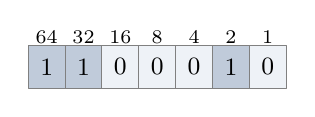
\begin{tikzpicture}[line join=round]
\node[,inner sep=1pt,font=\scriptsize] at (0.306,-0.252) {64};
\filldraw[draw=black!50,fill=FAUblue!25] (0.072,-0.360) rectangle (0.540,-0.900);
\node[,inner sep=1pt,font=\small] at (0.306,-0.630) {1};
\node[,inner sep=1pt,font=\scriptsize] at (0.774,-0.252) {32};
\filldraw[draw=black!50,fill=FAUblue!25] (0.540,-0.360) rectangle (1.008,-0.900);
\node[,inner sep=1pt,font=\small] at (0.774,-0.630) {1};
\node[,inner sep=1pt,font=\scriptsize] at (1.242,-0.252) {16};
\filldraw[draw=black!50,fill=Paperblue] (1.008,-0.360) rectangle (1.476,-0.900);
\node[,inner sep=1pt,font=\small] at (1.242,-0.630) {0};
\node[,inner sep=1pt,font=\scriptsize] at (1.710,-0.252) {8};
\filldraw[draw=black!50,fill=Paperblue] (1.476,-0.360) rectangle (1.944,-0.900);
\node[,inner sep=1pt,font=\small] at (1.710,-0.630) {0};
\node[,inner sep=1pt,font=\scriptsize] at (2.178,-0.252) {4};
\filldraw[draw=black!50,fill=Paperblue] (1.944,-0.360) rectangle (2.412,-0.900);
\node[,inner sep=1pt,font=\small] at (2.178,-0.630) {0};
\node[,inner sep=1pt,font=\scriptsize] at (2.646,-0.252) {2};
\filldraw[draw=black!50,fill=FAUblue!25] (2.412,-0.360) rectangle (2.880,-0.900);
\node[,inner sep=1pt,font=\small] at (2.646,-0.630) {1};
\node[,inner sep=1pt,font=\scriptsize] at (3.114,-0.252) {1};
\filldraw[draw=black!50,fill=Paperblue] (2.880,-0.360) rectangle (3.348,-0.900);
\node[,inner sep=1pt,font=\small] at (3.114,-0.630) {0};
\end{tikzpicture}\par\smallskip{\small\raggedright \textbf{(1100010)\textsubscript{2}}: add the place values above each 1: 64 + 32 + 2 = 98.\par}\end{minipage}
\end{center}

\begin{workedbox}{Worked conversion \ensuremath{\cdot} decimal to binary}
Convert 45 to binary by repeated division.

\Needspace{7\baselineskip}
\begin{enumerate}
\item 45 ÷ 2 gives quotient 22, remainder 1.
\item 22 ÷ 2 gives quotient 11, remainder 0; then 11 gives 5 remainder 1.
\item Continue: 5 gives 2 remainder 1; 2 gives 1 remainder 0; 1 gives 0 remainder 1.
\item Read remainders upward: 101101\textsubscript{2}. Check: 32+8+4+1=45. \hfill{\small\color{FAUblue}§3.1}
\end{enumerate}
\end{workedbox}
\end{keepsection}

\begin{keepsection}
\Needspace{14\baselineskip}
\subsection{Octal and hexadecimal}

\Needspace{11\baselineskip}
Because 8=2\textsuperscript{3}, each octal digit corresponds to three binary digits. Because 16=2\textsuperscript{4}, each hexadecimal digit corresponds to four bits. Group binary digits from the right and pad the leftmost group with zeroes if needed. In hexadecimal, A–F mean 10–15.

\begin{equationcard}{Compact binary groups}
\[ \begin{gathered} 10101_{2}\, =\, 010\, 101\, =\, 25_{8} \\ 10010100_{2}\, =\, 1001\, 0100\, =\, 94_{16} \\ 1\, \text{byte}\, =\, 8\, \text{bits}\, =\, 2\, \text{hexadecimal}\, \text{digits} \end{gathered} \]
{\small The lecture uses 16-bit words and 32-bit long words as examples; the sizes named by these terms can depend on a computer architecture.}
\end{equationcard}

\begin{workedbox}{Worked conversion \ensuremath{\cdot} hexadecimal to binary and decimal}
Convert 2F\textsubscript{16}.

\Needspace{5\baselineskip}
\begin{enumerate}
\item Replace each digit by four bits: 2 is 0010 and F (15) is 1111, so 2F\textsubscript{16}=0010 1111\textsubscript{2}.
\item Expand by base 16: 2\ensuremath{\times}16+15=47.
\item Check by the bits: 32+8+4+2+1=47. \hfill{\small\color{FAUblue}§3.1}
\end{enumerate}
\end{workedbox}

\Needspace{6\baselineskip}
\begin{notebox}\textbf{Trap:} do not read a binary string as an ordinary decimal integer. Attach its base, expand it, and only then compare values.\end{notebox}

\Needspace{5\baselineskip}
\begin{notebox}\textbf{Near miss:} 10\textsubscript{2} looks like ten, but in binary it is 1 \ensuremath{\cdot} 2 + 0 \ensuremath{\cdot} 1 = 2. Read the base before the digits.\end{notebox}

\Needspace{10\baselineskip}
\begin{recallbox}{Recall check \ensuremath{\cdot} answer without looking}
\Needspace{5\baselineskip}
\begin{enumerate}
\item What power of the base multiplies the rightmost digit?
\item Why can binary be grouped in threes to convert to octal?
\item What is A in hexadecimal worth in decimal?
\end{enumerate}

\nopagebreak[4]{\small\itshape Answers: see “3.1 Number systems and positional notation” under Answers at the end.}
\end{recallbox}
\end{keepsection}
\end{keepsection}

\begin{keepsection}
\Needspace{11\baselineskip}
\section{3.2 Integer representations}

\Needspace{8\baselineskip}
A computer stores a fixed number of bits, not a plus or minus sign unless the encoding defines one. The same pattern can mean different values under different encodings.

\begin{plainbox}\textbf{In plain words:} a computer stores only a row of bits; whether the row means a positive number, a negative number or something else depends on the agreed encoding. Unsigned uses every bit for size. The signed encodings give part of the range to negatives, and two’s complement, the one computers use, gives the top bit a negative weight.\end{plainbox}

\begin{keepsection}
\Needspace{17\baselineskip}
\subsection{Unsigned and signed ranges}

\Needspace{14\baselineskip}
An unsigned n-bit pattern represents 0 through 2\textsuperscript{n}\ensuremath{-}1. Signed encodings trade positive range for negative values. The source compares sign-and-magnitude, one’s complement, two’s complement, excess (biased) notation, and binary-coded decimal (BCD). The lecture judges a signed encoding by four wishes: one zero, a balanced range, simple fast addition hardware, and no gaps in the number line.

\begin{equationcard}{Ranges for n bits}
\[ \begin{gathered} \text{Unsigned}:\, 0\, …\, 2^{{n}}-1 \\ \text{Sign}\, \text{and}\, \text{magnitude}:\, -(2^{{n}-1}-1)\, …\, +(2^{{n}-1}-1) \\ \text{One}’\mathrm{s}\, \text{complement}:\, -(2^{{n}-1}-1)\, …\, +(2^{{n}-1}-1) \\ \text{Two}’\mathrm{s}\, \text{complement}:\, -2^{{n}-1}\, …\, 2^{{n}-1}-1 \end{gathered} \]
{\small \emph{Read it as: “with n bits, unsigned runs from 0 to 2\textsuperscript{n} \ensuremath{-} 1; two’s complement runs from \ensuremath{-}2\textsuperscript{n\ensuremath{-}1} to 2\textsuperscript{n\ensuremath{-}1} \ensuremath{-} 1”.}\par Sign-and-magnitude and one’s complement have two zero encodings. Two’s complement has one zero and one extra negative value.}
\end{equationcard}

\begin{workedbox}{Worked comparison \ensuremath{\cdot} decode 1111 in four encodings}
\Needspace{7\baselineskip}
\begin{enumerate}
\item Unsigned: 15.
\item Sign-and-magnitude: sign bit 1 and magnitude 111, so \ensuremath{-}7.
\item One’s complement: invert to 0000, so \ensuremath{-}0, which equals zero but has a distinct pattern.
\item Two’s complement: the unsigned value 15 represents 15\ensuremath{-}16=\ensuremath{-}1. \hfill{\small\color{FAUblue}§3.2}
\end{enumerate}
\end{workedbox}
\end{keepsection}

\begin{keepsection}
\Needspace{9\baselineskip}
\subsection{Why the older encodings lost}

Sign-and-magnitude has two zeros, and its adder must compare signs and then choose whether to add or subtract magnitudes. One’s complement still has two zeros, and its addition needs an end-around carry: a carry out of the top bit is added back into the lowest bit. For example, 0101 (+5) + 1110 (\ensuremath{-}1) gives 1 0011; adding the carry back gives 0100 (+4). Two’s complement has one zero and needs no such correction, at the price of a range that is not quite balanced.
\end{keepsection}

\begin{keepsection}
\Needspace{21\baselineskip}
\subsection{Two’s complement and bias}

\Needspace{18\baselineskip}
To form \ensuremath{-}x in n-bit two’s complement, invert all n bits of x and add 1; discard a carry beyond the width. The minimum value \ensuremath{-}2\textsuperscript{n\ensuremath{-}1} is the exception: its positive counterpart is outside the signed range, so fixed-width negation leaves the same pattern and overflows. Why inverting and adding one works: inverting x gives (2\textsuperscript{n}\ensuremath{-}1)\ensuremath{-}x, because each bit becomes 1 minus itself. Adding 1 gives 2\textsuperscript{n}\ensuremath{-}x, which is exactly the pattern for \ensuremath{-}x modulo 2\textsuperscript{n}. Equivalently, interpret a pattern with top bit 1 by subtracting 2\textsuperscript{n} from its unsigned value. In excess-B notation, actual value = stored unsigned value \ensuremath{-} B. The lecture’s three-bit excess-4 example therefore maps 000 to \ensuremath{-}4 and 111 to 3. Bias has a practical reason: the order of the true values matches the unsigned order of the stored patterns, so comparing two excess values is a plain unsigned comparison.

\begin{equationcard}{Decode rules}
\[ \begin{gathered} \text{Two}’\mathrm{s}-\text{complement}\, \text{value}\, =\, \text{unsigned}(\text{pattern})\, -\, 2^{{n}}\, \text{when}\, \text{the}\, \text{top}\, \text{bit}\, \text{is}\, 1 \\ \text{Negate}\, {x}:\, \text{invert}\, {n}\, \text{bits},\, \text{then}\, \text{add}\, 1 \\ \text{Excess}-\mathrm{B}\, \text{value}\, =\, \text{stored}\, \text{value}\, -\, {B} \end{gathered} \]
{\small \emph{Read it as: “when the top bit is 1, the two’s-complement value is the unsigned value minus 2\textsuperscript{n}”; to negate, flip every bit and add 1.}\par Keep the width fixed throughout. The same bit pattern has no signed meaning until an encoding is specified.}
\end{equationcard}

\Needspace{14\baselineskip}
\begin{center}
\begin{minipage}[t]{0.950\linewidth}\centering
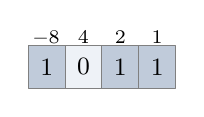
\begin{tikzpicture}[line join=round]
\node[,inner sep=1pt,font=\scriptsize] at (0.306,-0.252) {\ensuremath{-}8};
\filldraw[draw=black!50,fill=FAUblue!25] (0.072,-0.360) rectangle (0.540,-0.900);
\node[,inner sep=1pt,font=\small] at (0.306,-0.630) {1};
\node[,inner sep=1pt,font=\scriptsize] at (0.774,-0.252) {4};
\filldraw[draw=black!50,fill=Paperblue] (0.540,-0.360) rectangle (1.008,-0.900);
\node[,inner sep=1pt,font=\small] at (0.774,-0.630) {0};
\node[,inner sep=1pt,font=\scriptsize] at (1.242,-0.252) {2};
\filldraw[draw=black!50,fill=FAUblue!25] (1.008,-0.360) rectangle (1.476,-0.900);
\node[,inner sep=1pt,font=\small] at (1.242,-0.630) {1};
\node[,inner sep=1pt,font=\scriptsize] at (1.710,-0.252) {1};
\filldraw[draw=black!50,fill=FAUblue!25] (1.476,-0.360) rectangle (1.944,-0.900);
\node[,inner sep=1pt,font=\small] at (1.710,-0.630) {1};
\end{tikzpicture}\par\smallskip{\small\raggedright \textbf{Four-bit two’s complement}: the top bit weighs \ensuremath{-}8, so 1011 = \ensuremath{-}8 + 2 + 1 = \ensuremath{-}5.\par}\end{minipage}
\end{center}
\end{keepsection}

\begin{keepsection}
\Needspace{10\baselineskip}
\subsection{BCD stores decimal digits separately}

\Needspace{7\baselineskip}
In four-bit BCD, each decimal digit has its own four-bit code. For example, decimal 59 is 0101 1001 in BCD, while the ordinary binary value 59 is 00111011. BCD uses more bits but keeps each decimal digit directly readable.

\Needspace{6\baselineskip}
\begin{notebox}\textbf{Trap:} do not convert all BCD bits as one binary number. Decode each four-bit group as a decimal digit.\end{notebox}

\Needspace{5\baselineskip}
\begin{notebox}\textbf{Near miss:} +8 in four-bit two’s complement looks as if it should be 1000, but 1000 is \ensuremath{-}8: the range stops at +7, so +8 cannot be stored in four bits.\end{notebox}

\Needspace{10\baselineskip}
\begin{recallbox}{Recall check \ensuremath{\cdot} answer without looking}
\Needspace{5\baselineskip}
\begin{enumerate}
\item What is the four-bit two’s-complement range?
\item Why is the two’s-complement range asymmetric?
\item What is the BCD encoding of decimal 42?
\end{enumerate}

\nopagebreak[4]{\small\itshape Answers: see “3.2 Integer representations” under Answers at the end.}
\end{recallbox}
\end{keepsection}
\end{keepsection}

\begin{keepsection}
\Needspace{11\baselineskip}
\section{3.3 Character data}

\Needspace{8\baselineskip}
Numbers are not the only data stored as bits. A character encoding assigns numeric codes to letters, digits, punctuation, and control characters.

\begin{plainbox}\textbf{In plain words:} text is stored as numbers too: a character encoding is a table that gives every letter, digit and symbol a numeric code. 7-bit ASCII has 128 codes, enough for basic English; Unicode extends the table to the world’s scripts, and a byte encoding says how each code is written as bytes.\end{plainbox}

\begin{keepsection}
\Needspace{15\baselineskip}
\subsection{ASCII and Unicode}

\Needspace{12\baselineskip}
ASCII uses seven bits, giving 128 code values. The lecture describes eight-bit extensions that use the additional 128 patterns, but those upper values depend on the particular extension. Unicode assigns code points to characters across many writing systems; its first 128 code points match ASCII. A code point and its byte encoding are related but are not the same concept.

\begin{equationcard}{Character-code facts}
\[ \begin{gathered} 7-\text{bit}\, \text{ASCII}:\, 2^{7}\, =\, 128\, \text{code}\, \text{values} \\ \text{ASCII}\, \text{code}\, \text{points}:\, 0\, …\, 127 \end{gathered} \]
{\small \emph{Read it as: “7-bit ASCII has 2\textsuperscript{7} = 128 code values, numbered 0 to 127”.}\par The first 128 Unicode code points correspond to ASCII. Byte encodings represent code points as bytes by their own rules.}
\end{equationcard}

\Needspace{14\baselineskip}
\begin{center}
\begin{minipage}[t]{0.950\linewidth}\centering
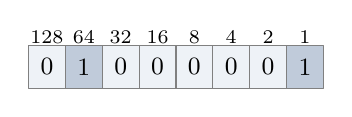
\begin{tikzpicture}[line join=round]
\node[,inner sep=1pt,font=\scriptsize] at (0.306,-0.252) {128};
\filldraw[draw=black!50,fill=Paperblue] (0.072,-0.360) rectangle (0.540,-0.900);
\node[,inner sep=1pt,font=\small] at (0.306,-0.630) {0};
\node[,inner sep=1pt,font=\scriptsize] at (0.774,-0.252) {64};
\filldraw[draw=black!50,fill=FAUblue!25] (0.540,-0.360) rectangle (1.008,-0.900);
\node[,inner sep=1pt,font=\small] at (0.774,-0.630) {1};
\node[,inner sep=1pt,font=\scriptsize] at (1.242,-0.252) {32};
\filldraw[draw=black!50,fill=Paperblue] (1.008,-0.360) rectangle (1.476,-0.900);
\node[,inner sep=1pt,font=\small] at (1.242,-0.630) {0};
\node[,inner sep=1pt,font=\scriptsize] at (1.710,-0.252) {16};
\filldraw[draw=black!50,fill=Paperblue] (1.476,-0.360) rectangle (1.944,-0.900);
\node[,inner sep=1pt,font=\small] at (1.710,-0.630) {0};
\node[,inner sep=1pt,font=\scriptsize] at (2.178,-0.252) {8};
\filldraw[draw=black!50,fill=Paperblue] (1.944,-0.360) rectangle (2.412,-0.900);
\node[,inner sep=1pt,font=\small] at (2.178,-0.630) {0};
\node[,inner sep=1pt,font=\scriptsize] at (2.646,-0.252) {4};
\filldraw[draw=black!50,fill=Paperblue] (2.412,-0.360) rectangle (2.880,-0.900);
\node[,inner sep=1pt,font=\small] at (2.646,-0.630) {0};
\node[,inner sep=1pt,font=\scriptsize] at (3.114,-0.252) {2};
\filldraw[draw=black!50,fill=Paperblue] (2.880,-0.360) rectangle (3.348,-0.900);
\node[,inner sep=1pt,font=\small] at (3.114,-0.630) {0};
\node[,inner sep=1pt,font=\scriptsize] at (3.582,-0.252) {1};
\filldraw[draw=black!50,fill=FAUblue!25] (3.348,-0.360) rectangle (3.816,-0.900);
\node[,inner sep=1pt,font=\small] at (3.582,-0.630) {1};
\end{tikzpicture}\par\smallskip{\small\raggedright \textbf{'A' in ASCII}: 0100 0001 = 64 + 1 = 65.\par}\end{minipage}
\end{center}

\begin{workedbox}{Worked encoding \ensuremath{\cdot} read a short ASCII string}
The lecture’s example encodes “Fred” in hexadecimal as 46 72 65 64.

\Needspace{5\baselineskip}
\begin{enumerate}
\item Split the bytes: 46, 72, 65, 64.
\item Read each as a hexadecimal ASCII code: 46 is F, 72 is r, 65 is e, and 64 is d.
\item The four codes decode to “Fred”. \hfill{\small\color{FAUblue}§3.3}
\end{enumerate}
\end{workedbox}

\Needspace{6\baselineskip}
\begin{notebox}\textbf{Trap:} an encoding is a mapping, not a property of the bit pattern by itself. Identify the character set and any byte encoding before decoding text.\end{notebox}

\Needspace{10\baselineskip}
\begin{notebox}\textbf{Near miss:} the character '7' looks like the number 7, but its ASCII code is 55. Arithmetic on character codes goes wrong unless you subtract the code of '0', which is 48, first.\end{notebox}

\begin{recallbox}{Recall check \ensuremath{\cdot} answer without looking}
\Needspace{4\baselineskip}
\begin{enumerate}
\item How many code values are available in seven-bit ASCII?
\item What is the relation between ASCII and the first 128 Unicode code points?
\end{enumerate}

\nopagebreak[4]{\small\itshape Answers: see “3.3 Character data” under Answers at the end.}
\end{recallbox}
\end{keepsection}
\end{keepsection}

\begin{keepsection}
\Needspace{11\baselineskip}
\section{3.4 Unsigned binary arithmetic}

\Needspace{8\baselineskip}
Binary arithmetic follows the same place-value logic as decimal arithmetic. Carries and borrows move between columns, while the fixed bit width limits which values can be stored.

\begin{plainbox}\textbf{In plain words:} binary arithmetic works column by column like the decimal method from school, only the columns are worth 1, 2, 4, 8, …. 1 + 1 makes 2, which is written 0 with 1 carried. The difference is that a computer has a fixed number of columns, so a carry out of the last column is lost.\end{plainbox}

\begin{keepsection}
\Needspace{13\baselineskip}
\subsection{Add and subtract}

\Needspace{10\baselineskip}
Add each column and carry 1 when a column totals 2. For subtraction, borrow from a higher column when the current minuend bit is too small; a borrowed binary 1 is worth 2 in the current column. Subtraction can also be checked by adding the difference to the subtrahend.

\begin{workedbox}{Worked addition \ensuremath{\cdot} include the carry}
Add 111011\textsubscript{2} and 101010\textsubscript{2}.

\Needspace{5\baselineskip}
\begin{enumerate}
\item From right to left: 1+0=1.
\item 1+1=10, so write 0 and carry 1. Continue each column with its carry.
\item The result is 1100101\textsubscript{2}. Check: 59+42=101, and 1100101\textsubscript{2}=101. \hfill{\small\color{FAUblue}§3.4}
\end{enumerate}
\end{workedbox}

\begin{workedbox}{Worked subtraction \ensuremath{\cdot} borrow across a zero}
Calculate 1010\textsubscript{2}\ensuremath{-}0011\textsubscript{2}.

\Needspace{9\baselineskip}
\begin{enumerate}
\item Rightmost column: 0\ensuremath{-}1 needs a borrow from the next column, so 2\ensuremath{-}1=1, and that column’s 1 becomes 0.
\item Next column: 0\ensuremath{-}1 needs a borrow, but the column to its left is 0, so take from the top bit. The top bit becomes 0, the third column keeps 1, and this column gets 2: 2\ensuremath{-}1=1.
\item Third column: 1\ensuremath{-}0=1. Top column: 0\ensuremath{-}0=0.
\item The result is 0111\textsubscript{2}. Check: 10\ensuremath{-}3=7. \hfill{\small\color{FAUblue}§3.4}
\end{enumerate}
\end{workedbox}
\end{keepsection}

\begin{keepsection}
\Needspace{14\baselineskip}
\subsection{Multiply and divide}

\Needspace{11\baselineskip}
Binary multiplication uses partial products, like decimal long multiplication, but each multiplier bit is only 0 or 1. Binary division uses quotient and remainder. For divisor d\ensuremath{\neq}0, dividend = quotient\ensuremath{\times}divisor + remainder, where 0\ensuremath{\leq}remainder\ensuremath{<}divisor.

\begin{equationcard}{Division check}
\[ \begin{gathered} \text{dividend}\, =\, \text{quotient}\, \times \, \text{divisor}\, +\, \text{remainder} \\ 0\, \leq \, \text{remainder}\, <\, \text{divisor} \end{gathered} \]
{\small \emph{Read it as: “dividend equals quotient times divisor plus remainder, with the remainder at least 0 and smaller than the divisor”.}\par Substitute the quotient, divisor, and remainder to check a division result.}
\end{equationcard}

\begin{workedbox}{Worked multiplication \ensuremath{\cdot} partial products}
Calculate 1101\textsubscript{2}\ensuremath{\times}101\textsubscript{2}.

\Needspace{7\baselineskip}
\begin{enumerate}
\item Multiplier bit 1 (rightmost): write 1101.
\item Multiplier bit 0: the partial product is zero.
\item Multiplier bit 1 (two places left): write 110100.
\item Add: 1101+110100=1000001\textsubscript{2}. Check: 13\ensuremath{\times}5=65. \hfill{\small\color{FAUblue}§3.4}
\end{enumerate}
\end{workedbox}

\begin{workedbox}{Worked division \ensuremath{\cdot} long division}
Calculate 10111\textsubscript{2}÷11\textsubscript{2}.

\Needspace{7\baselineskip}
\begin{enumerate}
\item 10 is smaller than 11, so take 101: quotient bit 1, remainder 101\ensuremath{-}11=10.
\item Bring down 1 to get 101: quotient bit 1, remainder 10.
\item Bring down 1 to get 101: quotient bit 1, remainder 10.
\item Quotient 111\textsubscript{2}, remainder 10\textsubscript{2}. Check: 7\ensuremath{\times}3+2=23. \hfill{\small\color{FAUblue}§3.4}
\end{enumerate}
\end{workedbox}

\Needspace{6\baselineskip}
\begin{notebox}\textbf{Memory hook:} in binary addition, 1+1 writes 0 and carries 1. In subtraction, a borrow makes the current column worth 2 before subtracting.\end{notebox}

\Needspace{5\baselineskip}
\begin{notebox}\textbf{Near miss:} in four bits, 1100 + 0101 gives the correct sum 10001, but only four bits are kept: 0001. The column arithmetic was right; the result just does not fit.\end{notebox}

\Needspace{9\baselineskip}
\begin{recallbox}{Recall check \ensuremath{\cdot} answer without looking}
\Needspace{4\baselineskip}
\begin{enumerate}
\item What bit do you write for 1+1, and what do you carry?
\item What inequality must the remainder satisfy?
\end{enumerate}

\nopagebreak[4]{\small\itshape Answers: see “3.4 Unsigned binary arithmetic” under Answers at the end.}
\end{recallbox}
\end{keepsection}
\end{keepsection}

\begin{keepsection}
\Needspace{12\baselineskip}
\section{3.5 Two’s-complement arithmetic and overflow}

\Needspace{9\baselineskip}
Two’s complement lets the same adder perform signed addition and subtraction. Correct bit operations still need a range check: a fixed-width result can wrap to a pattern with a different signed value.

\begin{plainbox}\textbf{In plain words:} two’s complement lets one adder handle both signs: to subtract, add the negation. The catch is the fixed range. Adding two positive numbers can go past the largest value and wrap round to a pattern that reads as negative. That is \textbf{overflow}, and it is not the same thing as a carry out of the top bit.\end{plainbox}

\begin{keepsection}
\Needspace{17\baselineskip}
\subsection{Addition, subtraction, and overflow}

\Needspace{14\baselineskip}
Add the bit patterns and discard any carry beyond the most significant bit. For subtraction, negate the subtrahend and add it to the minuend. Signed overflow occurs when the exact mathematical result lies outside the representation’s range. For addition, it occurs when two operands with the same sign produce a result with the opposite sign; operands of unlike signs cannot overflow.

\begin{equationcard}{n-bit two’s-complement checks}
\[ \begin{gathered} \text{Range}:\, -2^{{n}-1}\, …\, 2^{{n}-1}-1 \\ {A}\, -\, {B}\, =\, {A}\, +\, (\text{two}’\mathrm{s}-\text{complement}\, \text{negation}\, \text{of}\, {B}) \\ \text{Same}-\text{sign}\, \text{addition}\, \text{with}\, \text{opposite}-\text{sign}\, \text{result}\, \Rightarrow \, \text{overflow} \end{gathered} \]
{\small \emph{Read it as: “A minus B is A plus the negation of B”; overflow on addition means two operands of the same sign gave a result of the other sign.}\par Discarding carry-out is part of fixed-width addition. Carry-out alone does not signal signed overflow.}
\end{equationcard}

\Needspace{14\baselineskip}
\begin{center}
\begin{minipage}[t]{0.950\linewidth}\centering
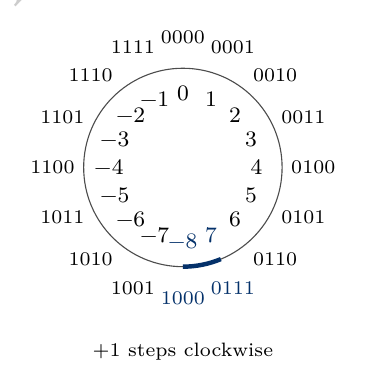
\begin{tikzpicture}[line join=round]
\draw[black!70] (2.160,-2.160) circle (1.260);
\node[,inner sep=1pt,font=\scriptsize] at (2.160,-0.504) {0000};
\node[,inner sep=1pt,font=\footnotesize] at (2.160,-1.224) {0};
\node[,inner sep=1pt,font=\scriptsize] at (2.794,-0.630) {0001};
\node[,inner sep=1pt,font=\footnotesize] at (2.518,-1.295) {1};
\node[,inner sep=1pt,font=\scriptsize] at (3.331,-0.989) {0010};
\node[,inner sep=1pt,font=\footnotesize] at (2.822,-1.498) {2};
\node[,inner sep=1pt,font=\scriptsize] at (3.690,-1.526) {0011};
\node[,inner sep=1pt,font=\footnotesize] at (3.025,-1.802) {3};
\node[,inner sep=1pt,font=\scriptsize] at (3.816,-2.160) {0100};
\node[,inner sep=1pt,font=\footnotesize] at (3.096,-2.160) {4};
\node[,inner sep=1pt,font=\scriptsize] at (3.690,-2.794) {0101};
\node[,inner sep=1pt,font=\footnotesize] at (3.025,-2.518) {5};
\node[,inner sep=1pt,font=\scriptsize] at (3.331,-3.331) {0110};
\node[,inner sep=1pt,font=\footnotesize] at (2.822,-2.822) {6};
\node[text=FAUblue,inner sep=1pt,font=\scriptsize] at (2.794,-3.690) {0111};
\node[text=FAUblue,inner sep=1pt,font=\footnotesize] at (2.518,-3.025) {7};
\node[text=FAUblue,inner sep=1pt,font=\scriptsize] at (2.160,-3.816) {1000};
\node[text=FAUblue,inner sep=1pt,font=\footnotesize] at (2.160,-3.096) {\ensuremath{-}8};
\node[,inner sep=1pt,font=\scriptsize] at (1.526,-3.690) {1001};
\node[,inner sep=1pt,font=\footnotesize] at (1.802,-3.025) {\ensuremath{-}7};
\node[,inner sep=1pt,font=\scriptsize] at (0.989,-3.331) {1010};
\node[,inner sep=1pt,font=\footnotesize] at (1.498,-2.822) {\ensuremath{-}6};
\node[,inner sep=1pt,font=\scriptsize] at (0.630,-2.794) {1011};
\node[,inner sep=1pt,font=\footnotesize] at (1.295,-2.518) {\ensuremath{-}5};
\node[,inner sep=1pt,font=\scriptsize] at (0.504,-2.160) {1100};
\node[,inner sep=1pt,font=\footnotesize] at (1.224,-2.160) {\ensuremath{-}4};
\node[,inner sep=1pt,font=\scriptsize] at (0.630,-1.526) {1101};
\node[,inner sep=1pt,font=\footnotesize] at (1.295,-1.802) {\ensuremath{-}3};
\node[,inner sep=1pt,font=\scriptsize] at (0.989,-0.989) {1110};
\node[,inner sep=1pt,font=\footnotesize] at (1.498,-1.498) {\ensuremath{-}2};
\node[,inner sep=1pt,font=\scriptsize] at (1.526,-0.630) {1111};
\node[,inner sep=1pt,font=\footnotesize] at (1.802,-1.295) {\ensuremath{-}1};
\draw[FAUblue,line width=1.6pt] ([shift={(-67.50:1.260)}]2.160,-2.160) arc (-67.50:-90.00:1.260);
\node[,inner sep=1pt,font=\scriptsize] at (2.160,-4.500) {+1 steps clockwise};
\end{tikzpicture}\par\smallskip{\small\raggedright \textbf{The 4-bit two’s-complement wheel}: adding 1 to 0111 (7) steps clockwise to 1000, which reads as \ensuremath{-}8. That jump at the bottom of the wheel is overflow.\par}\end{minipage}
\end{center}

\begin{workedbox}{Worked example \ensuremath{\cdot} detect overflow}
Use four-bit two’s complement to calculate \ensuremath{-}7+(\ensuremath{-}6).

\Needspace{6\baselineskip}
\begin{enumerate}
\item Encode \ensuremath{-}7 as 1001 and \ensuremath{-}6 as 1010.
\item Add: 1001+1010=1 0011. Discard the carry-out, leaving 0011.
\item The stored result 0011 is +3, but the exact sum is \ensuremath{-}13, outside the four-bit range \ensuremath{-}8…+7. Both inputs were negative and the result is positive, so overflow occurred. \hfill{\small\color{FAUblue}§3.5}
\end{enumerate}
\end{workedbox}
\end{keepsection}

\begin{keepsection}
\Needspace{17\baselineskip}
\subsection{Multiplication and division}

\Needspace{14\baselineskip}
The lecture notes that ordinary unsigned multiplication cannot simply be applied to signed two’s-complement patterns and read at the original width. A full product may require up to twice as many bits as the operands; retain a sufficient width and interpret the result consistently. For a simple signed multiplication, multiply magnitudes and make the result negative exactly when the operand signs differ, then check the available width. The supplied slides introduce this idea but do not give a complete signed division algorithm.

\begin{workedbox}{Worked multiplication \ensuremath{\cdot} signed values}
Calculate (\ensuremath{-}3)\ensuremath{\times}(+5) and store it in eight-bit two’s complement.

\Needspace{7\baselineskip}
\begin{enumerate}
\item Multiply magnitudes: 3\ensuremath{\times}5=15=00001111\textsubscript{2}.
\item The signs differ, so the result is negative.
\item Negate in eight bits: invert to 11110000 and add 1, giving 11110001.
\item Check: 241\ensuremath{-}256=\ensuremath{-}15, inside \ensuremath{-}128…+127. Four bits could not hold it. \hfill{\small\color{FAUblue}§3.5}
\end{enumerate}
\end{workedbox}

\Needspace{7\baselineskip}
Overflow also matters for safety. The lecture warns that an integer overflow in a memory-size calculation can become a security hole, such as a buffer overflow, because too little memory gets allocated.

\Needspace{7\baselineskip}
\begin{notebox}\textbf{Sign check:} do not treat discarded carry as overflow. Decode the fixed-width result and compare it with the exact mathematical result and allowed range.\end{notebox}

\Needspace{6\baselineskip}
\begin{notebox}\textbf{Near miss:} in four bits, 0111 + 0001 = 1000 has no carry out of the top bit, yet it is wrong: 7 + 1 = 8 is out of range, and 1000 reads as \ensuremath{-}8. Overflow is judged by the signs, not by the carry.\end{notebox}

\Needspace{11\baselineskip}
\begin{recallbox}{Recall check \ensuremath{\cdot} answer without looking}
\Needspace{5\baselineskip}
\begin{enumerate}
\item How is A\ensuremath{-}B implemented in two’s-complement arithmetic?
\item Can two’s-complement addition overflow when the operands have unlike signs?
\item Why can a signed product need more bits than either input?
\end{enumerate}

\nopagebreak[4]{\small\itshape Answers: see “3.5 Two’s-complement arithmetic and overflow” under Answers at the end.}
\end{recallbox}
\end{keepsection}
\end{keepsection}

\begin{keepsection}
\Needspace{13\baselineskip}
\section{4.1 The floating-point model}

\Needspace{10\baselineskip}
Fixed-width integers from §3.5 cannot hold fractions or very large and very small values. Floating point uses a sign, a significand, and an exponent to cover those magnitudes, at the cost of exactness.

\begin{plainbox}\textbf{In plain words:} a floating-point number is scientific notation in binary: a sign, a short run of significant digits (the \textbf{significand}) and an \textbf{exponent} that slides the point left or right. A fixed number of bits holds only so many significant digits, so most real numbers are stored as the nearest value the format can hold, and the gaps between neighbouring values grow as the numbers get larger.\end{plainbox}

\begin{keepsection}
\Needspace{9\baselineskip}
\subsection{Range and precision}

\Needspace{6\baselineskip}
For base β, a normalised number has the form sign \ensuremath{\times} significand \ensuremath{\times} β\textsuperscript{exponent}. The exponent controls scale and therefore the approximate range. The number of significand bits controls precision, or how finely nearby values can be distinguished.

\Needspace{9\baselineskip}
Floating-point values are finite in number, and their spacing changes with magnitude.

\begin{equationcard}{Scientific notation model}
\[ \begin{gathered} {x}\, =\, {s}\, \times \, {M}\, \times \, β^{{E}} \end{gathered} \]
{\small \emph{Read it as: “x is s times M times β to the E”: the sign s, the significand M with the digits, and the exponent E that says where the point goes.}\par s is the sign, M is the significand, β is the base or radix, and E is the exponent. In binary floating point, β=2.}
\end{equationcard}

\Needspace{14\baselineskip}
\begin{center}
\begin{minipage}[t]{0.950\linewidth}\centering
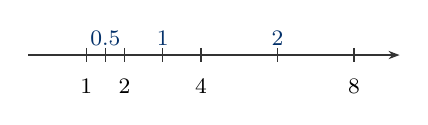
\begin{tikzpicture}[line join=round]
\draw[-{Stealth[length=4pt]},black!80] (0.180,-0.612) -- (4.896,-0.612);
\draw[black!80] (0.918,-0.522) -- (0.918,-0.702);
\node[,inner sep=1pt,font=\footnotesize] at (0.918,-1.008) {1};
\draw[black!80] (1.160,-0.522) -- (1.160,-0.702);
\draw[black!80] (1.403,-0.522) -- (1.403,-0.702);
\node[,inner sep=1pt,font=\footnotesize] at (1.403,-1.008) {2};
\draw[black!80] (1.889,-0.522) -- (1.889,-0.702);
\draw[black!80] (2.374,-0.522) -- (2.374,-0.702);
\node[,inner sep=1pt,font=\footnotesize] at (2.374,-1.008) {4};
\draw[black!80] (3.345,-0.522) -- (3.345,-0.702);
\draw[black!80] (4.317,-0.522) -- (4.317,-0.702);
\node[,inner sep=1pt,font=\footnotesize] at (4.317,-1.008) {8};
\node[text=FAUblue,inner sep=1pt,font=\footnotesize] at (1.160,-0.396) {0.5};
\node[text=FAUblue,inner sep=1pt,font=\footnotesize] at (1.889,-0.396) {1};
\node[text=FAUblue,inner sep=1pt,font=\footnotesize] at (3.345,-0.396) {2};
\end{tikzpicture}\par\smallskip{\small\raggedright \textbf{Gaps double} with 2 significant bits: the values 1, 1.5, then 2, 3, then 4, 6, 8 lie 0.5, then 1, then 2 apart (the numbers above each zone).\par}\end{minipage}
\end{center}

\begin{equationcard}{Local gap between neighbours}
\[ \begin{gathered} \text{gap}\, \text{within}\, [2^{{E}},\, 2^{{E}+1})\, =\, 2^{{E}-{p}+1} \end{gathered} \]
{\small \emph{Read it as: “the gap between neighbouring values in [2\textsuperscript{E}, 2\textsuperscript{E+1}) is 2\textsuperscript{E\ensuremath{-}p+1}”: it doubles every time the values cross a power of 2.}\par p is the number of significand bits. (This follows directly from the notes’ model: the last of p bits has weight 2\textsuperscript{\ensuremath{-}(p\ensuremath{-}1)}, scaled by 2\textsuperscript{E}. The notes only say the gap grows.) Between 8 and 16, E=3, so p=24 gives 2\textsuperscript{\ensuremath{-}20}.}
\end{equationcard}

\begin{workedbox}{Worked example \ensuremath{\cdot} normalise a decimal value}
Write 343000 \ensuremath{\times} 10\textsuperscript{\ensuremath{-}4} in normalised decimal form with 1\ensuremath{\leq}M\ensuremath{<}10.

\Needspace{5\baselineskip}
\begin{enumerate}
\item Move the decimal point in 343000 five places left to make 3.43.
\item Increase the exponent by five to preserve the value: 3.43 \ensuremath{\times} 10\textsuperscript{1}.
\item Check: 343000 \ensuremath{\times} 10\textsuperscript{\ensuremath{-}4}=34.3, and 3.43 \ensuremath{\times} 10\textsuperscript{1}=34.3. \hfill{\small\color{FAUblue}§4.1}
\end{enumerate}
\end{workedbox}

\Needspace{7\baselineskip}
\begin{notebox}\textbf{Trap:} moving the radix point changes the exponent in the opposite direction if the represented value is to stay the same.\end{notebox}

\Needspace{6\baselineskip}
\begin{notebox}\textbf{Near miss:} 12.5 \ensuremath{\times} 10\textsuperscript{0} and 1.25 \ensuremath{\times} 10\textsuperscript{1} are the same number, but only the second is normalised, with one non-zero digit before the point. A format that allowed both would spend bit patterns on duplicate values.\end{notebox}

\Needspace{11\baselineskip}
\begin{recallbox}{Recall check \ensuremath{\cdot} answer without looking}
\Needspace{5\baselineskip}
\begin{enumerate}
\item Which field chiefly determines range?
\item Which field chiefly determines precision?
\item Why are floating-point values not evenly spaced over the number line?
\end{enumerate}

\nopagebreak[4]{\small\itshape Answers: see “4.1 The floating-point model” under Answers at the end.}
\end{recallbox}
\end{keepsection}
\end{keepsection}

\begin{keepsection}
\Needspace{10\baselineskip}
\section{4.2 Binary fractions}

\Needspace{7\baselineskip}
The significand from §4.1 is a binary fraction, so its place values explain both conversion and approximation.

\Needspace{7\baselineskip}
\begin{plainbox}\textbf{In plain words:} binary fractions work like decimal ones with halves instead of tenths: after the binary point the places are worth 1/2, 1/4, 1/8, …. Some fractions that are short in decimal never end in binary, just as 1/3 never ends in decimal.\end{plainbox}

The first bit after the binary point has weight 2\textsuperscript{\ensuremath{-}1}, and each following bit has half the previous weight.

\begin{keepsection}
\Needspace{10\baselineskip}
\subsection{Convert binary fractions to decimal}

\begin{equationcard}{Binary fractional place values}
\[ \begin{gathered} 0.{b}_{1}{b}_{2}…{b}_{{k}}\, =\, {b}_{1}2^{-1}\, +\, {b}_{2}2^{-2}\, +\, …\, +\, {b}_{{k}}2^{-{k}} \end{gathered} \]
{\small \emph{Read it as: “0.b\textsubscript{1}b\textsubscript{2}…b\textsubscript{k} is b\textsubscript{1} halves plus b\textsubscript{2} quarters plus …”: each bit times its power of one half.}\par Each b\textsubscript{i} is 0 or 1. A leading integer part is evaluated with non-negative powers of 2.}
\end{equationcard}

\Needspace{14\baselineskip}
\begin{center}
\begin{minipage}[t]{0.950\linewidth}\centering
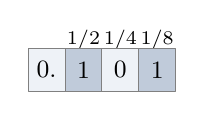
\begin{tikzpicture}[line join=round]
\filldraw[draw=black!50,fill=Paperblue] (0.072,-0.360) rectangle (0.540,-0.900);
\node[,inner sep=1pt,font=\small] at (0.306,-0.630) {0.};
\node[,inner sep=1pt,font=\scriptsize] at (0.774,-0.252) {1/2};
\filldraw[draw=black!50,fill=FAUblue!25] (0.540,-0.360) rectangle (1.008,-0.900);
\node[,inner sep=1pt,font=\small] at (0.774,-0.630) {1};
\node[,inner sep=1pt,font=\scriptsize] at (1.242,-0.252) {1/4};
\filldraw[draw=black!50,fill=Paperblue] (1.008,-0.360) rectangle (1.476,-0.900);
\node[,inner sep=1pt,font=\small] at (1.242,-0.630) {0};
\node[,inner sep=1pt,font=\scriptsize] at (1.710,-0.252) {1/8};
\filldraw[draw=black!50,fill=FAUblue!25] (1.476,-0.360) rectangle (1.944,-0.900);
\node[,inner sep=1pt,font=\small] at (1.710,-0.630) {1};
\end{tikzpicture}\par\smallskip{\small\raggedright \textbf{0.101\textsubscript{2}} = 1/2 + 1/8 = 0.625: each place after the point is worth half the one before.\par}\end{minipage}
\end{center}

\begin{workedbox}{Worked conversion \ensuremath{\cdot} binary fraction to decimal}
Convert 0.01101\textsubscript{2} to decimal.

\Needspace{5\baselineskip}
\begin{enumerate}
\item Use the five place values: 1/2, 1/4, 1/8, 1/16, and 1/32.
\item Keep the places where the bit is 1: 1/4 + 1/8 + 1/32.
\item Add: 0.25+0.125+0.03125=0.40625. \hfill{\small\color{FAUblue}§4.2}
\end{enumerate}
\end{workedbox}
\end{keepsection}

\begin{keepsection}
\Needspace{8\baselineskip}
\subsection{Convert decimal fractions to binary}

\Needspace{5\baselineskip}
Repeatedly multiply the fractional part by 2.

\Needspace{11\baselineskip}
At each step, the integer part is the next binary digit, and the new fractional part is carried into the next step.

\begin{workedbox}{Worked conversion \ensuremath{\cdot} terminating binary fraction}
Convert 0.6875 to binary.

\Needspace{8\baselineskip}
\begin{enumerate}
\item 0.6875\ensuremath{\times}2=1.375, so the first bit is 1; carry 0.375.
\item 0.375\ensuremath{\times}2=0.75, so the next bit is 0; carry 0.75.
\item 0.75\ensuremath{\times}2=1.5, so the next bit is 1; carry 0.5.
\item 0.5\ensuremath{\times}2=1.0, so the next bit is 1; the fraction is now zero.
\item Therefore 0.6875=0.1011\textsubscript{2}. Check: 1/2+1/8+1/16=0.6875. \hfill{\small\color{FAUblue}§4.2}
\end{enumerate}
\end{workedbox}

\Needspace{4\baselineskip}
Some fractions, such as 0.1 in decimal, repeat in binary.

\Needspace{4\baselineskip}
A finite significand stores only an approximation of a repeating expansion.

\Needspace{6\baselineskip}
\begin{notebox}\textbf{Trap:} a decimal fraction that looks short is not necessarily exact in binary.\end{notebox}

\Needspace{6\baselineskip}
\begin{notebox}\textbf{Near miss:} 0.1 has a single digit in decimal, but in binary it is 0.000110011… with the block 0011 repeating forever, so a computer can only store an approximation. 0.5 = 0.1\textsubscript{2}, by contrast, is exact.\end{notebox}

\Needspace{10\baselineskip}
\begin{recallbox}{Recall check \ensuremath{\cdot} answer without looking}
\Needspace{5\baselineskip}
\begin{enumerate}
\item What is the weight of the fourth binary digit after the point?
\item What is 0.101\textsubscript{2} in decimal?
\item Why can a computer store 0.1 only approximately in binary floating point?
\end{enumerate}

\nopagebreak[4]{\small\itshape Answers: see “4.2 Binary fractions” under Answers at the end.}
\end{recallbox}
\end{keepsection}
\end{keepsection}

\begin{keepsection}
\Needspace{10\baselineskip}
\section{4.3 Floating-point arithmetic and error}

\Needspace{7\baselineskip}
The exponent and significand must be managed during each operation.

\Needspace{8\baselineskip}
\begin{plainbox}\textbf{In plain words:} to multiply two floating-point numbers, multiply the significands and add the exponents. To add them, first shift the one with the smaller exponent until the exponents match, then add. Either way the result is normalised and rounded, and that rounding is where small errors creep in.\end{plainbox}

After the exact operation, the result may need normalisation and rounding to fit the available precision.

\begin{keepsection}
\Needspace{9\baselineskip}
\subsection{Multiplication}

\begin{equationcard}{Multiply normalised values}
\[ \begin{gathered} ({M}_{1}\, \times \, β^{{E}_{1}})({M}_{2}\, \times \, β^{{E}_{2}})\, =\, ({M}_{1}{M}_{2})\, \times \, β^{{E}_{1}+{E}_{2}} \end{gathered} \]
{\small Multiply the significands and add the exponents. Then normalise and round if needed.}
\end{equationcard}

\begin{workedbox}{Worked multiplication \ensuremath{\cdot} normalise the result}
Calculate (2.6\ensuremath{\times}10\textsuperscript{3})(5.4\ensuremath{\times}10\textsuperscript{\ensuremath{-}2}).

\Needspace{5\baselineskip}
\begin{enumerate}
\item Multiply significands: 2.6\ensuremath{\times}5.4=14.04.
\item Add exponents: 3+(\ensuremath{-}2)=1, giving 14.04\ensuremath{\times}10\textsuperscript{1}.
\item Normalise: 1.404\ensuremath{\times}10\textsuperscript{2}=140.4. \hfill{\small\color{FAUblue}§4.3}
\end{enumerate}
\end{workedbox}
\end{keepsection}

\begin{keepsection}
\Needspace{8\baselineskip}
\subsection{Addition}

\Needspace{5\baselineskip}
Before adding, express both numbers with the same exponent.

\Needspace{5\baselineskip}
Shift the significand of the value with the smaller exponent to the right by the exponent difference.

\Needspace{10\baselineskip}
This alignment can discard low-order digits before the addition is even performed.

\begin{workedbox}{Worked addition \ensuremath{\cdot} align exponents}
Use two significant decimal digits to add 4.5\ensuremath{\times}10\textsuperscript{3} and 6.7\ensuremath{\times}10\textsuperscript{2}.

\Needspace{6\baselineskip}
\begin{enumerate}
\item Rewrite the second value at exponent 3: 6.7\ensuremath{\times}10\textsuperscript{2}=0.67\ensuremath{\times}10\textsuperscript{3}.
\item Add significands: (4.5+0.67)\ensuremath{\times}10\textsuperscript{3}=5.17\ensuremath{\times}10\textsuperscript{3}.
\item Round to two significant digits: 5.2\ensuremath{\times}10\textsuperscript{3}. The exact sum is 5170, while this two-digit result is 5200. \hfill{\small\color{FAUblue}§4.3}
\end{enumerate}
\end{workedbox}
\end{keepsection}

\begin{keepsection}
\Needspace{7\baselineskip}
\subsection{Rounding, overflow, and comparison}

\Needspace{4\baselineskip}
Truncation drops extra digits and tends to bias results in one direction.

\Needspace{4\baselineskip}
Rounding chooses a nearby representable value and usually gives a better approximation.

\Needspace{4\baselineskip}
Exponent overflow occurs when the result is too large for the format.

\Needspace{5\baselineskip}
Exponent underflow occurs when the result is too small for the normalised range.

\Needspace{5\baselineskip}
The slides describe infinity or an exception for overflow, and zero or an exception for underflow in their simplified model.

\Needspace{5\baselineskip}
IEEE formats also provide subnormal numbers near zero.

\Needspace{10\baselineskip}
For approximate comparisons, choose a tolerance ε that fits the scale and precision of the problem.

\begin{equationcard}{Absolute tolerance example}
\[ \begin{gathered} \text{Treat}\, {a}\, \text{as}\, \text{close}\, \text{to}\, {b}\, \text{when}\, |{a}-{b}|\, <\, ε \\ \text{For}\, {b}\, =\, 1\, \text{and}\, ε\, =\, 0.000005:\, 0.999995\, <\, {a}\, <\, 1.000005 \end{gathered} \]
{\small \emph{Read it as: “treat a as close to b when the distance between them is less than ε”.}\par A fixed absolute tolerance may be unsuitable when magnitudes vary greatly. The slides also introduce relative closeness.}
\end{equationcard}

\Needspace{6\baselineskip}
\begin{notebox}\textbf{Sign check:} estimate the order of magnitude before accepting a rounded result.\end{notebox}

\Needspace{6\baselineskip}
\begin{notebox}\textbf{Near miss:} 0.1 + 0.2 looks as if it should equal 0.3, but in double precision the computed sum is 0.30000000000000004, so the test 0.1 + 0.2 == 0.3 is false. Compare floating-point results with a tolerance instead.\end{notebox}

\Needspace{13\baselineskip}
\begin{recallbox}{Recall check \ensuremath{\cdot} answer without looking}
\Needspace{7\baselineskip}
\begin{enumerate}
\item What do you do to the exponents when multiplying?
\item Which operand’s significand is shifted to align an addition?
\item How do overflow and underflow differ?
\item Why can direct equality comparison be unreliable for computed floating-point values?
\end{enumerate}

\nopagebreak[4]{\small\itshape Answers: see “4.3 Floating-point arithmetic and error” under Answers at the end.}
\end{recallbox}
\end{keepsection}
\end{keepsection}

\begin{keepsection}
\Needspace{10\baselineskip}
\section{4.4 IEEE 754 binary formats}

\Needspace{7\baselineskip}
A shared format defines how floating-point fields are stored and how arithmetic behaves.

\Needspace{8\baselineskip}
\begin{plainbox}\textbf{In plain words:} IEEE 754 is the shared recipe for storing a floating-point number: one sign bit, an exponent field stored with an offset (the \textbf{bias}) so it needs no sign of its own, and the fraction bits after the binary point. A normalised number always starts with 1., so that 1 is not stored at all: it is the \textbf{hidden bit}.\end{plainbox}

The slides introduce IEEE 754 as a widely adopted standard for predictable binary floating-point arithmetic.

\begin{keepsection}
\Needspace{10\baselineskip}
\subsection{Single and double precision}

\Needspace{10\baselineskip}
\begin{center}\small\begin{tabularx}{\linewidth}{>{\raggedright\arraybackslash}X>{\raggedright\arraybackslash}X>{\raggedright\arraybackslash}X>{\raggedright\arraybackslash}X>{\raggedright\arraybackslash}X>{\raggedright\arraybackslash}X>{\raggedright\arraybackslash}X}\toprule
\textbf{Format} & \textbf{Total} & \textbf{Sign} & \textbf{Exponent} & \textbf{Fraction field} & \textbf{Significand precision} & \textbf{Bias} \\ \midrule
Single & 32 bits & 1 bit & 8 bits & 23 bits & 24 bits for normal values & 127 \\
Double & 64 bits & 1 bit & 11 bits & 52 bits & 53 bits for normal values & 1023 \\
\bottomrule\end{tabularx}\end{center}

\Needspace{6\baselineskip}
For a normalised binary value, the leading significand bit is 1 and is omitted from the stored fraction field.

\Needspace{11\baselineskip}
The exponent field stores a biased exponent rather than a two’s-complement exponent. Stored order then matches true order, so hardware can compare two exponents as plain unsigned integers.

\begin{equationcard}{Normalised value rule}
\[ \begin{gathered} \text{value}\, =\, (-1)^{{S}}\, \times \, 1.{F}\, \times \, 2^{{E}-\text{bias}} \\ \text{Single}\, \text{bias}\, =\, 127 \\ \text{double}\, \text{bias}\, =\, 1023 \end{gathered} \]
{\small \emph{Read it as: “value is \ensuremath{-}1 to the S, times 1.F, times 2 to the (E minus bias)”: the sign, the stored fraction with its hidden 1, and the exponent once the bias is removed.}\par S is the sign bit, E is the unsigned exponent field, and F is the stored fraction interpreted after the binary point. This rule is for normalised values.}
\end{equationcard}

\Needspace{14\baselineskip}
\begin{center}
\begin{minipage}[t]{0.950\linewidth}\centering
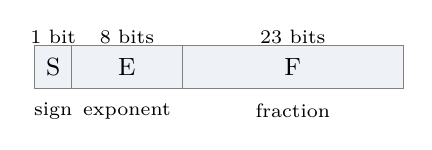
\begin{tikzpicture}[line join=round]
\node[,inner sep=1pt,font=\scriptsize] at (0.306,-0.252) {1 bit};
\filldraw[draw=black!50,fill=Paperblue] (0.072,-0.360) rectangle (0.540,-0.900);
\node[,inner sep=1pt,font=\small] at (0.306,-0.630) {S};
\node[,inner sep=1pt,font=\scriptsize] at (0.306,-1.188) {sign};
\node[,inner sep=1pt,font=\scriptsize] at (1.242,-0.252) {8 bits};
\filldraw[draw=black!50,fill=Paperblue] (0.540,-0.360) rectangle (1.944,-0.900);
\node[,inner sep=1pt,font=\small] at (1.242,-0.630) {E};
\node[,inner sep=1pt,font=\scriptsize] at (1.242,-1.188) {exponent};
\node[,inner sep=1pt,font=\scriptsize] at (3.348,-0.252) {23 bits};
\filldraw[draw=black!50,fill=Paperblue] (1.944,-0.360) rectangle (4.752,-0.900);
\node[,inner sep=1pt,font=\small] at (3.348,-0.630) {F};
\node[,inner sep=1pt,font=\scriptsize] at (3.348,-1.188) {fraction};
\end{tikzpicture}\par\smallskip{\small\raggedright \textbf{IEEE 754 single precision}: 1 sign bit, 8 exponent bits stored with bias 127, and 23 fraction bits after the hidden 1, 32 bits in all.\par}\end{minipage}
\end{center}
\end{keepsection}

\begin{keepsection}
\Needspace{11\baselineskip}
\subsection{Convert decimal to single precision}

\begin{workedbox}{Worked conversion \ensuremath{\cdot} 42.6875}
\Needspace{8\baselineskip}
\begin{enumerate}
\item Convert to binary: 42.6875=101010.1011\textsubscript{2}.
\item Normalise: 1.010101011\ensuremath{\times}2\textsuperscript{5}, so the sign bit is 0.
\item Store the fraction after the hidden leading 1: 01010101100000000000000.
\item Bias the exponent: 5+127=132=10000100\textsubscript{2}.
\item The fields are 0 | 10000100 | 01010101100000000000000, or hexadecimal 422A C000. \hfill{\small\color{FAUblue}§4.4}
\end{enumerate}
\end{workedbox}
\end{keepsection}

\begin{keepsection}
\Needspace{10\baselineskip}
\subsection{Decode single precision}

\begin{workedbox}{Worked decoding \ensuremath{\cdot} BEC0 0000}
\Needspace{7\baselineskip}
\begin{enumerate}
\item The sign bit is 1, so the value is negative.
\item The exponent field is 01111101\textsubscript{2}=125; subtract the bias: 125\ensuremath{-}127=\ensuremath{-}2.
\item Restore the hidden bit: 1.1000…\textsubscript{2}=1.5.
\item Scale: 1.5\ensuremath{\times}2\textsuperscript{\ensuremath{-}2}=0.375. Apply the sign: \ensuremath{-}0.375. \hfill{\small\color{FAUblue}§4.4}
\end{enumerate}
\end{workedbox}

\Needspace{6\baselineskip}
\begin{notebox}\textbf{Trap:} restore the hidden leading 1 when decoding a normalised value, but do not apply that rule to a subnormal value.\end{notebox}

\Needspace{5\baselineskip}
\begin{notebox}\textbf{Near miss:} the single-precision exponent field 10000000 looks like a large exponent, but it means 128 \ensuremath{-} 127 = 1. Subtract the bias before reading the exponent.\end{notebox}

\Needspace{11\baselineskip}
\begin{recallbox}{Recall check \ensuremath{\cdot} answer without looking}
\Needspace{6\baselineskip}
\begin{enumerate}
\item How many bits are stored in the single-precision fraction field?
\item What is the single-precision exponent bias?
\item Why can a normalised value have 24 bits of significand precision while storing only 23 fraction bits?
\end{enumerate}

\nopagebreak[4]{\small\itshape Answers: see “4.4 IEEE 754 binary formats” under Answers at the end.}
\end{recallbox}
\end{keepsection}
\end{keepsection}

\begin{keepsection}
\Needspace{10\baselineskip}
\section{4.5 Zero, subnormal numbers, infinity, and NaN}

\Needspace{7\baselineskip}
Reserved exponent patterns extend useful behaviour beyond normalised values.

\Needspace{14\baselineskip}
\begin{center}
\begin{minipage}[t]{0.303\linewidth}\centering
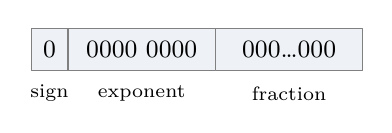
\begin{tikzpicture}[line join=round]
\filldraw[draw=black!50,fill=Paperblue] (0.072,-0.360) rectangle (0.540,-0.900);
\node[,inner sep=1pt,font=\small] at (0.306,-0.630) {0};
\node[,inner sep=1pt,font=\scriptsize] at (0.306,-1.188) {sign};
\filldraw[draw=black!50,fill=Paperblue] (0.540,-0.360) rectangle (2.412,-0.900);
\node[,inner sep=1pt,font=\small] at (1.476,-0.630) {0000 0000};
\node[,inner sep=1pt,font=\scriptsize] at (1.476,-1.188) {exponent};
\filldraw[draw=black!50,fill=Paperblue] (2.412,-0.360) rectangle (4.284,-0.900);
\node[,inner sep=1pt,font=\small] at (3.348,-0.630) {000…000};
\node[,inner sep=1pt,font=\scriptsize] at (3.348,-1.188) {fraction};
\end{tikzpicture}\par\smallskip{\small\raggedright \textbf{+0}: every bit is 0.\par}\end{minipage}\hfill
\begin{minipage}[t]{0.303\linewidth}\centering
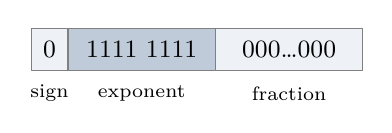
\begin{tikzpicture}[line join=round]
\filldraw[draw=black!50,fill=Paperblue] (0.072,-0.360) rectangle (0.540,-0.900);
\node[,inner sep=1pt,font=\small] at (0.306,-0.630) {0};
\node[,inner sep=1pt,font=\scriptsize] at (0.306,-1.188) {sign};
\filldraw[draw=black!50,fill=FAUblue!25] (0.540,-0.360) rectangle (2.412,-0.900);
\node[,inner sep=1pt,font=\small] at (1.476,-0.630) {1111 1111};
\node[,inner sep=1pt,font=\scriptsize] at (1.476,-1.188) {exponent};
\filldraw[draw=black!50,fill=Paperblue] (2.412,-0.360) rectangle (4.284,-0.900);
\node[,inner sep=1pt,font=\small] at (3.348,-0.630) {000…000};
\node[,inner sep=1pt,font=\scriptsize] at (3.348,-1.188) {fraction};
\end{tikzpicture}\par\smallskip{\small\raggedright \textbf{+\ensuremath{\infty}}: exponent all 1s, fraction 0.\par}\end{minipage}\hfill
\begin{minipage}[t]{0.303\linewidth}\centering
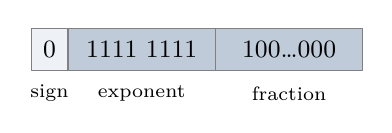
\begin{tikzpicture}[line join=round]
\filldraw[draw=black!50,fill=Paperblue] (0.072,-0.360) rectangle (0.540,-0.900);
\node[,inner sep=1pt,font=\small] at (0.306,-0.630) {0};
\node[,inner sep=1pt,font=\scriptsize] at (0.306,-1.188) {sign};
\filldraw[draw=black!50,fill=FAUblue!25] (0.540,-0.360) rectangle (2.412,-0.900);
\node[,inner sep=1pt,font=\small] at (1.476,-0.630) {1111 1111};
\node[,inner sep=1pt,font=\scriptsize] at (1.476,-1.188) {exponent};
\filldraw[draw=black!50,fill=FAUblue!25] (2.412,-0.360) rectangle (4.284,-0.900);
\node[,inner sep=1pt,font=\small] at (3.348,-0.630) {100…000};
\node[,inner sep=1pt,font=\scriptsize] at (3.348,-1.188) {fraction};
\end{tikzpicture}\par\smallskip{\small\raggedright \textbf{NaN}: exponent all 1s, fraction not 0.\par}\end{minipage}
\end{center}

\Needspace{7\baselineskip}
\begin{plainbox}\textbf{In plain words:} some exponent patterns are kept for special cases. An exponent of all zeros means zero or a tiny \textbf{subnormal} number that fills the gap just above zero; an exponent of all ones means infinity when the fraction is zero, and NaN, “not a number”, for results such as 0/0.\end{plainbox}

\Needspace{14\baselineskip}
In single precision, exponent field zero and exponent field all ones have special interpretations.

\Needspace{10\baselineskip}
\begin{center}\small\begin{tabularx}{\linewidth}{>{\raggedright\arraybackslash}X>{\raggedright\arraybackslash}X>{\raggedright\arraybackslash}X}\toprule
\textbf{Exponent field} & \textbf{Fraction field} & \textbf{Meaning} \\ \midrule
All zeroes & All zeroes & Positive or negative zero \\
All zeroes & Non-zero & Subnormal number \\
Neither all zeroes nor all ones & Any pattern & Normalised number \\
All ones & All zeroes & Positive or negative infinity \\
All ones & Non-zero & NaN, or not-a-number \\
\bottomrule\end{tabularx}\end{center}

\begin{equationcard}{Subnormal value rule}
\[ \begin{gathered} \text{value}\, =\, (-1)^{{S}}\, \times \, 0.{F}\, \times \, 2^{-126} \\ \text{Smallest}\, \text{normal}\, \text{single}:\, 2^{-126}\, \approx \, 1.175\times 10^{-38} \end{gathered} \]
{\small \emph{Read it as: “a subnormal value is \ensuremath{-}1 to the S times 0.F times 2\textsuperscript{\ensuremath{-}126}”: no hidden 1, and the exponent stays at its smallest value.}\par For a subnormal single-precision number, the hidden bit is 0 and the exponent is fixed at \ensuremath{-}126. Precision falls as the value nears zero.}
\end{equationcard}

\Needspace{8\baselineskip}
Subnormal values fill the gap between the smallest normal value and zero, so underflow is gradual. They also keep the property x\ensuremath{-}y==0 exactly when x==y, even for very small numbers.

\Needspace{8\baselineskip}
They can be slow: many CPUs handle them through a microcode assist or a software trap, which the lecture calls orders of magnitude slower. Flush-to-zero (FTZ) is a non-compliant mode that treats subnormals as zero. It is faster but gives up that correctness, and high-performance programs often enable it.

\Needspace{6\baselineskip}
Infinity represents overflow results and some divisions by zero. NaN represents an operation without a real-number result, such as 0/0, \ensuremath{\surd}\ensuremath{-}1 or infinity\ensuremath{-}infinity.

\Needspace{6\baselineskip}
Before IEEE 754, such operations could trap and end the program. With these values the computation continues, and the status propagates to be checked later.

Operations on infinity and NaN follow format rules, not ordinary real-number algebra in every case.

\begin{keepsection}
\Needspace{17\baselineskip}
\subsection{Special arithmetic examples}

\Needspace{10\baselineskip}
\begin{center}\small\begin{tabularx}{\linewidth}{>{\raggedright\arraybackslash}X>{\raggedright\arraybackslash}X}\toprule
\textbf{Operation} & \textbf{Result} \\ \midrule
N ÷ \ensuremath{\pm}\ensuremath{\infty} & 0 \\
\ensuremath{\pm} non-zero ÷ 0 & \ensuremath{\pm}\ensuremath{\infty} \\
+\ensuremath{\infty} + +\ensuremath{\infty} & +\ensuremath{\infty} \\
\ensuremath{\infty} + 5.0 & \ensuremath{\infty} \\
\ensuremath{\pm}\ensuremath{\infty} \ensuremath{\times} \ensuremath{\pm}\ensuremath{\infty} & \ensuremath{\pm}\ensuremath{\infty} \\
\ensuremath{\pm}0 ÷ \ensuremath{\pm}0 & NaN \\
+\ensuremath{\infty} \ensuremath{-} +\ensuremath{\infty} & NaN \\
\ensuremath{\pm}\ensuremath{\infty} ÷ \ensuremath{\pm}\ensuremath{\infty} & NaN \\
\ensuremath{\pm}\ensuremath{\infty} \ensuremath{\times} 0 & NaN \\
\bottomrule\end{tabularx}\end{center}

\Needspace{10\baselineskip}
The sign of the infinity in signed cases depends on the operand signs. An invalid operation normally returns a quiet NaN; a trap may be enabled instead.

\begin{workedbox}{Worked classification \ensuremath{\cdot} single precision fields}
Classify sign 0, exponent 11111111, fraction 000…000.

\Needspace{5\baselineskip}
\begin{enumerate}
\item The exponent field is all ones.
\item The fraction field is all zeroes.
\item This encodes positive infinity. \hfill{\small\color{FAUblue}§4.5}
\end{enumerate}
\end{workedbox}

\begin{notebox}\textbf{Trap:} an all-ones exponent does not always mean infinity; inspect the fraction field to distinguish infinity from NaN.\end{notebox}
\end{keepsection}

\begin{keepsection}
\Needspace{7\baselineskip}
\subsection{Numerical stability and cancellation}

Cancellation occurs when subtracting close stored values. The subtraction may itself be exact, yet earlier rounding in the operands can dominate the small difference. A stable method avoids needlessly creating that sensitive subtraction.
\end{keepsection}

\begin{keepsection}
\Needspace{15\baselineskip}
\subsection{Machine epsilon and relative error}

\Needspace{12\baselineskip}
Machine epsilon is the gap from 1 to the next larger representable value. For radix β and p significant digits, ε\textsubscript{mach}=β\textsuperscript{1\ensuremath{-}p}. Here p counts the full significand digits, including the hidden leading bit in a normalised IEEE value.

\begin{equationcard}{Binary machine epsilon}
\[ \begin{gathered} \text{Single}\, \text{precision}:\, {p}\, =\, 24,\, ε_{\text{mach}}\, =\, 2^{-23}\, \approx \, 1.19\times 10^{-7} \\ \text{Double}\, \text{precision}:\, {p}\, =\, 53,\, ε_{\text{mach}}\, =\, 2^{-52}\, \approx \, 2.22\times 10^{-16} \end{gathered} \]
{\small \emph{Read it as: “ε\textsubscript{mach} is the gap between 1 and the next larger value the format can store”: 2\textsuperscript{\ensuremath{-}23} in single precision.}\par Under round-to-nearest, the unit roundoff u is ε\textsubscript{mach}/2 for normal results. “Unit roundoff” is not a term from the slides.}
\end{equationcard}

\begin{equationcard}{Relative rounding model}
\[ \begin{gathered} \text{fl}({x})\, =\, {x}(1+δ),\, \text{with}\, |δ|\, \leq \, {u} \end{gathered} \]
{\small \emph{Read it as: “the stored value fl(x) is x times (1 + δ), with |δ| at most u”: rounding changes a number by a small relative amount.}\par For finite non-zero normal results, round-to-nearest, and no overflow. Relative error is measured against |x|, so the same absolute error matters more when the true answer is small.}
\end{equationcard}

\Needspace{10\baselineskip}
The slides bound the error by ε; under round-to-nearest the tight bound is ε/2 (= u). Both statements are true; use the slide form if the exam asks for it.

\begin{equationcard}{Error propagation in a difference}
\[ \begin{gathered} {x}′\, =\, {x}(1+δ_{{x}}),\, {y}′\, =\, {y}(1+δ_{{y}}) \\ \text{relative}\, \text{error}\, =\, (({x}′-{y}′)-({x}-{y}))/({x}-{y})\, =\, ({x}δ_{{x}}-{y}δ_{{y}})/({x}-{y}) \end{gathered} \]
{\small The numerator stays about the size of the input errors. As x approaches y the denominator approaches zero, so the relative error can explode.}
\end{equationcard}

\begin{workedbox}{Worked example \ensuremath{\cdot} cancellation}
Suppose five significant decimal digits store x=0.123456789 as 0.12346 and y=0.123451234 as 0.12345.

\Needspace{6\baselineskip}
\begin{enumerate}
\item The exact difference is 0.000005555.
\item The stored difference is 0.00001.
\item The stored difference is about 1.80 times the exact difference, so its relative error is about 80.0\%. The subtraction exposed input rounding error. \hfill{\small\color{FAUblue}§4.5}
\end{enumerate}
\end{workedbox}
\end{keepsection}

\begin{keepsection}
\Needspace{8\baselineskip}
\subsection{Sterbenz lemma}

If x and y are positive finite floating-point values in the same radix and precision, and y/2\ensuremath{\leq}x\ensuremath{\leq}2y, then x\ensuremath{-}y is exactly representable when gradual underflow is supported. For example, 1.5 and 1.0 meet the condition, and their difference 0.5 is exact. This does not undo rounding that happened while x or y was computed; cancellation can expose that earlier error.
\end{keepsection}

\begin{keepsection}
\Needspace{13\baselineskip}
\subsection{Stable quadratic roots}

\Needspace{10\baselineskip}
For ax\textsuperscript{2}+bx+c=0, require a\ensuremath{\neq}0 and D=b\textsuperscript{2}\ensuremath{-}4ac\ensuremath{\geq}0. The usual formula can subtract nearly equal quantities for one root. For D\ensuremath{>}0, choose the branch that adds magnitudes: if b\ensuremath{\geq}0, set q=\ensuremath{-}\ensuremath{\tfrac12}(b+\ensuremath{\surd}D); if b\ensuremath{<}0, set q=\ensuremath{-}\ensuremath{\tfrac12}(b\ensuremath{-}\ensuremath{\surd}D). Then the roots are q/a and c/q. This branch also handles b=0. For D=0, use the repeated root \ensuremath{-}b/(2a), since q may be zero. These steps avoid cancellation while respecting the degenerate cases.

\Needspace{12\baselineskip}
The notes write the same method as x\textsubscript{1}=(\ensuremath{-}b\ensuremath{-}sgn(b)\ensuremath{\surd}D)/(2a) and x\textsubscript{2}=c/(a x\textsubscript{1}). Since q=a\ensuremath{\cdot}x\textsubscript{1}, c/q is the slide’s c/(a x\textsubscript{1}). The second form comes from expanding a(x\ensuremath{-}x\textsubscript{1})(x\ensuremath{-}x\textsubscript{2}): matching the constant term gives x\textsubscript{1}x\textsubscript{2}=c/a, which is Vieta’s relation, so x\textsubscript{2} needs no subtraction.

\begin{workedbox}{Worked example \ensuremath{\cdot} x\textsuperscript{2}+10\textsuperscript{8}x+1=0 in double precision}
\Needspace{9\baselineskip}
\begin{enumerate}
\item Here a=1, b=10\textsuperscript{8}, c=1, so D=10\textsuperscript{16}\ensuremath{-}4 and \ensuremath{\surd}D\ensuremath{\approx}10\textsuperscript{8}.
\item Direct formula for the small root: (\ensuremath{-}b+\ensuremath{\surd}D)/2 subtracts nearly equal values and gives about \ensuremath{-}7.45\ensuremath{\times}10\textsuperscript{\ensuremath{-}9}.
\item Stable: b\ensuremath{\geq}0, so q=\ensuremath{-}\ensuremath{\tfrac12}(b+\ensuremath{\surd}D)\ensuremath{\approx}\ensuremath{-}10\textsuperscript{8}. The roots are q/a\ensuremath{\approx}\ensuremath{-}10\textsuperscript{8} and c/q\ensuremath{\approx}\ensuremath{-}10\textsuperscript{\ensuremath{-}8}.
\item Check: the product of the roots is 1=c/a, and the sum is about \ensuremath{-}10\textsuperscript{8}=\ensuremath{-}b/a. The direct value was about 25\% off. \hfill{\small\color{FAUblue}§4.5}
\end{enumerate}
\end{workedbox}

\begin{notebox}\textbf{Trap:} mathematical equivalence does not guarantee equal numerical accuracy. Look for subtraction of nearly equal values and avoid rounding intermediate results unnecessarily.\end{notebox}
\end{keepsection}

\begin{keepsection}
\Needspace{14\baselineskip}
\subsection{Fused multiply-add}

\Needspace{11\baselineskip}
A fused multiply-add evaluates a\ensuremath{\times}b+c with one final rounding. Separate multiplication and addition can round the product first, then round again after addition. FMA can therefore preserve more information; its speed benefit depends on hardware. The lecture names dot products, matrix multiplication and polynomial evaluation as algorithms that gain from it.

\begin{equationcard}{Fused versus separate rounding}
\[ \begin{gathered} \text{FMA}({a},{b},{c})\, =\, \text{round}({a}\times {b}+{c}) \\ \text{Separate}:\, \text{round}(\text{round}({a}\times {b})+{c}) \end{gathered} \]
{\small The fused operation avoids the intermediate rounding step.}
\end{equationcard}

\Needspace{5\baselineskip}
\begin{notebox}\textbf{Near miss:} +0 and \ensuremath{-}0 have different bit patterns and compare as equal, yet they are not interchangeable: 1/(+0) gives +\ensuremath{\infty} while 1/(\ensuremath{-}0) gives \ensuremath{-}\ensuremath{\infty}. The sign bit still matters at zero.\end{notebox}

\Needspace{14\baselineskip}
\begin{recallbox}{Recall check \ensuremath{\cdot} answer without looking}
\Needspace{8\baselineskip}
\begin{enumerate}
\item How do you distinguish infinity from NaN?
\item What is the main purpose of subnormal numbers?
\item What does zero exponent and zero fraction encode?
\item What does machine epsilon measure, and how is it related to the unit roundoff?
\item Which quadratic root should you compute second, and how?
\end{enumerate}

\nopagebreak[4]{\small\itshape Answers: see “4.5 Zero, subnormal numbers, infinity, and NaN” under Answers at the end.}
\end{recallbox}
\end{keepsection}
\end{keepsection}

\begin{keepsection}
\Needspace{11\baselineskip}
\section{5.1 C memory and pointers}

\Needspace{8\baselineskip}
Everything so far gave meaning to bit patterns. C also lets you handle where those patterns live, because an address is itself a number you can store. That gives direct control and direct ways to fail.

\begin{plainbox}\textbf{In plain words:} every variable lives at an address in memory, and in C that address is a value you can store: a \textbf{pointer}. \& gives the address of a variable, and * follows an address to the value stored there. That gives direct control over memory, and direct ways to break it.\end{plainbox}

\begin{keepsection}
\Needspace{15\baselineskip}
\subsection{Addresses, \& and *}

\Needspace{12\baselineskip}
C treats memory as a contiguous line of bytes, each with a numerical address, usually written in hexadecimal. A pointer is a variable that stores an address. The operator \& gives the address of a variable, and * reads or writes the value at an address.

\begin{equationcard}{Core syntax}
\[ \begin{gathered} \text{int}\, *\mathrm{p};\, \text{declares}\, \mathrm{a}\, \text{pointer}\, \text{to}\, \text{int} \\ \text{int}\, \mathrm{x}\, =\, 10;\, \mathrm{p}\, =\, \&\mathrm{x};\, \mathrm{p}\, \text{now}\, \text{holds}\, \text{the}\, \text{address}\, \text{of}\, \mathrm{x} \\ *{p}\, =\, 20 \\ \text{writes}\, \text{through}\, {p},\, \text{so}\, {x}\, \text{becomes}\, 20 \end{gathered} \]
{\small \emph{Read it as: “int *p declares p as a pointer to an int”; “p = \&x puts the address of x into p”; “*p = 20 writes 20 wherever p points”.}\par In a declaration, * builds a pointer type. In an expression, * dereferences.}
\end{equationcard}

\Needspace{14\baselineskip}
\begin{center}
\begin{minipage}[t]{0.950\linewidth}\centering
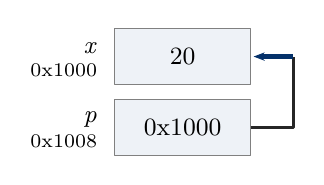
\begin{tikzpicture}[line join=round]
\node[anchor=east,inner sep=1pt,font=\small] at (1.800,-0.432) {\textit{x}};
\node[anchor=east,inner sep=1pt,font=\scriptsize] at (1.800,-0.720) {0x1000};
\draw[black!50,fill=Paperblue] (1.980,-0.180) rectangle (3.708,-0.900);
\node[,inner sep=1pt,font=\small] at (2.844,-0.540) {20};
\node[anchor=east,inner sep=1pt,font=\small] at (1.800,-1.332) {\textit{p}};
\node[anchor=east,inner sep=1pt,font=\scriptsize] at (1.800,-1.620) {0x1008};
\draw[black!50,fill=Paperblue] (1.980,-1.080) rectangle (3.708,-1.800);
\node[,inner sep=1pt,font=\small] at (2.844,-1.440) {0x1000};
\draw[black!85,line width=1pt] (3.708,-1.440) -- (4.248,-1.440) -- (4.248,-0.540);
\draw[-{Stealth[length=4pt]},FAUblue,line width=1.6pt] (4.248,-0.540) -- (3.744,-0.540);
\end{tikzpicture}\par\smallskip{\small\raggedright \textbf{A pointer}: p stores the address of x, so *p = 20 writes into x. The addresses are illustrative.\par}\end{minipage}
\end{center}
\end{keepsection}

\begin{keepsection}
\Needspace{13\baselineskip}
\subsection{Pointer arithmetic and arrays}

\Needspace{10\baselineskip}
Adding n to a pointer moves n elements, not n bytes. In most expressions an array name decays to a pointer to its first element, and subscripting is defined through that pointer.

\begin{equationcard}{Scaling and subscripts}
\[ \begin{gathered} \text{new}\, \text{address}\, =\, \text{old}\, \text{address}\, +\, \mathrm{n}\, \times \, \text{sizeof}(\text{type}) \\ {a}[{i}]\, \text{means}\, *({a}\, +\, {i}) \end{gathered} \]
{\small \emph{Read it as: “adding n to a pointer moves it n elements, that is n \ensuremath{\times} sizeof(type) bytes, not n bytes”; a[i] is the same as *(a + i).}\par Sizes depend on the platform; the lecture assumes 4 bytes for int and 8 for double.}
\end{equationcard}

\begin{workedbox}{Worked example \ensuremath{\cdot} scaled steps}
With int a[10]; int *p = \&a[0]; the array starts at 0x1000, and sizeof(int) is 4.

\Needspace{6\baselineskip}
\begin{enumerate}
\item p+1 is 0x1000+1\ensuremath{\times}4=0x1004, the address of a[1].
\item p+3 is 0x1000+3\ensuremath{\times}4=0x100C, because 12 is C in hexadecimal. This is the address of a[3].
\item For struct Point \{ double x; double y; \} each element takes 2\ensuremath{\times}8=16 bytes, so the same +1 step moves 16 bytes. Check: the step always equals the element size. \hfill{\small\color{FAUblue}§5.1}
\end{enumerate}
\end{workedbox}

A function that receives an array actually receives a copy of the pointer to its first element. That is why arrays appear to be passed by reference.
\end{keepsection}

\begin{keepsection}
\Needspace{14\baselineskip}
\subsection{Double pointers and function pointers}

\Needspace{11\baselineskip}
C passes every argument by value, so a function given a pointer gets a copy and cannot change the caller’s pointer. To let it do so, as an allocating function must, pass the address of the pointer. A pointer to a pointer adds one level of indirection: with int **p2 = \&p1; *p2 is p1 and **p2 is the int.

\begin{equationcard}{Changing the caller’s pointer}
\[ \begin{gathered} \text{void}\, \text{allocate}(\text{int}\, **\text{ptr},\, \text{int}\, \text{size})\, \{\, *\text{ptr}\, =\, \text{malloc}(\text{size}\, *\, \text{sizeof}(\text{int}));\, \} \\ \text{int}\, *\text{my}\, =\, \text{NULL};\, \text{allocate}(\&\text{my},\, 10); \end{gathered} \]
{\small Inside the function, *ptr is the caller’s my itself.}
\end{equationcard}

\begin{equationcard}{Function pointers}
\[ \begin{gathered} \text{int}\, (*\text{op})(\text{int},\, \text{int})\, =\, \text{add};\, \text{result}\, =\, (*\text{op})(5,\, 3); \end{gathered} \]
{\small A pointer can hold the address of code. Passing one to another function gives a callback, as in qsort or event handlers. With add returning a+b, result is 8.}
\end{equationcard}
\end{keepsection}

\begin{keepsection}
\Needspace{15\baselineskip}
\subsection{Pitfalls}

\Needspace{10\baselineskip}
\begin{center}\small\begin{tabularx}{\linewidth}{>{\raggedright\arraybackslash}X>{\raggedright\arraybackslash}X>{\raggedright\arraybackslash}X}\toprule
\textbf{Problem} & \textbf{What goes wrong} & \textbf{Habit} \\ \midrule
Uninitialised pointer & Holds a garbage address; writing through it is undefined behaviour. & Initialise: p = NULL or p = \&some\_variable. \\
NULL dereference & Undefined behaviour; a crash such as a segmentation fault is typical. & Test p != NULL first. \\
Memory leak & The only pointer to a malloc block is lost, so it can never be freed. & Pair each malloc with a free. \\
Dangling pointer & The pointer still holds the address of freed memory, which may be reused. & free(p); p = NULL; \\
\bottomrule\end{tabularx}\end{center}

\Needspace{7\baselineskip}
\begin{notebox}\textbf{Trap:} setting p to NULL after free only protects that one pointer. Any other copy of the address still dangles.\end{notebox}

\Needspace{13\baselineskip}
\begin{notebox}\textbf{Near miss:} after int *p = malloc(sizeof(int)); free(p); the pointer p still holds the old address, and *p may even still show the old value, but reading it is undefined behaviour: that memory no longer belongs to you.\end{notebox}

\begin{recallbox}{Recall check \ensuremath{\cdot} answer without looking}
\Needspace{5\baselineskip}
\begin{enumerate}
\item If q is a double pointer value 0x2000 with 8-byte double, what is q+2?
\item Why must an allocating function take int ** rather than int *?
\item What is a dangling pointer?
\end{enumerate}

\nopagebreak[4]{\small\itshape Answers: see “5.1 C memory and pointers” under Answers at the end.}
\end{recallbox}
\end{keepsection}
\end{keepsection}

\begin{keepsection}
\Needspace{12\baselineskip}
\section{5.2 The Python memory model}

\Needspace{9\baselineskip}
Python keeps the reference idea from §5.1 but hides the addresses and the freeing. Knowing the model tells you when a change through one name shows up through another.

\Needspace{14\baselineskip}
\begin{center}
\begin{minipage}[t]{0.950\linewidth}\centering
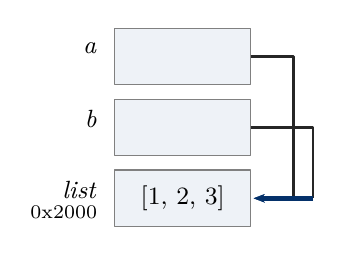
\begin{tikzpicture}[line join=round]
\node[anchor=east,inner sep=1pt,font=\small] at (1.800,-0.432) {\textit{a}};
\draw[black!50,fill=Paperblue] (1.980,-0.180) rectangle (3.708,-0.900);
\node[,inner sep=1pt,font=\small] at (2.844,-0.540) {};
\node[anchor=east,inner sep=1pt,font=\small] at (1.800,-1.332) {\textit{b}};
\draw[black!50,fill=Paperblue] (1.980,-1.080) rectangle (3.708,-1.800);
\node[,inner sep=1pt,font=\small] at (2.844,-1.440) {};
\node[anchor=east,inner sep=1pt,font=\small] at (1.800,-2.232) {\textit{list}};
\node[anchor=east,inner sep=1pt,font=\scriptsize] at (1.800,-2.520) {0x2000};
\draw[black!50,fill=Paperblue] (1.980,-1.980) rectangle (3.708,-2.700);
\node[,inner sep=1pt,font=\small] at (2.844,-2.340) {[1, 2, 3]};
\draw[black!85,line width=1pt] (3.708,-0.540) -- (4.248,-0.540) -- (4.248,-2.340);
\draw[-{Stealth[length=4pt]},FAUblue,line width=1.6pt] (4.248,-2.340) -- (3.744,-2.340);
\draw[black!85,line width=1pt] (3.708,-1.440) -- (4.500,-1.440) -- (4.500,-2.340);
\draw[-{Stealth[length=4pt]},FAUblue,line width=1.6pt] (4.500,-2.340) -- (3.744,-2.340);
\end{tikzpicture}\par\smallskip{\small\raggedright \textbf{Two names, one list}: after b = a, both names refer to the same object, so a += [3] changes what b sees too. The address is illustrative.\par}\end{minipage}
\end{center}

\begin{plainbox}\textbf{In plain words:} in Python a variable is a name tag tied to an object, not a box that holds a value. b = a ties a second tag to the same object. If the object can change, as a list can, a change made through one name shows up through the other; if it cannot, as a number or a string cannot, “changing” it really ties the name to a new object.\end{plainbox}

\begin{keepsection}
\Needspace{17\baselineskip}
\subsection{Names, objects and rebinding}

\Needspace{14\baselineskip}
A C variable is a typed box that holds a value. A Python variable is a name bound to an object that lives elsewhere, and all data, including integers and functions, are objects. The built-in id() gives an object’s identifier, which in CPython is its memory address, so you can see when two names share an object. In C, x = 20 overwrites the box. In Python, x = 20 rebinds the name to another object and leaves the old object unchanged.

\begin{workedbox}{Worked trace \ensuremath{\cdot} shared reference then rebinding}
Trace a = [1, 2, 3]; b = a; b.append(4); b = [0]; print(a).

\Needspace{8\baselineskip}
\begin{enumerate}
\item a = [1, 2, 3] makes one list object and binds a to it.
\item b = a binds a second name to the same object, so id(a) equals id(b).
\item b.append(4) changes that object, so a now shows [1, 2, 3, 4].
\item b = [0] rebinds b only. print(a) gives [1, 2, 3, 4]. Check: exactly one statement changed the object a refers to. \hfill{\small\color{FAUblue}§5.2}
\end{enumerate}
\end{workedbox}
\end{keepsection}

\begin{keepsection}
\Needspace{11\baselineskip}
\subsection{Mutability and function arguments}

\Needspace{8\baselineskip}
Immutable objects (int, float, str, tuple) cannot change after creation, so operations make new objects. Mutable objects (list, dict, set) can change in place, and the change is visible through every name that refers to them.

A function receives a reference to the object, which is called pass-by-object-reference. It cannot change what the caller’s name refers to, but it can change a mutable object’s contents. With data = [1, 2, 3], a function calling some\_list.append(4) leaves data as [1, 2, 3, 4].
\end{keepsection}

\begin{keepsection}
\Needspace{21\baselineskip}
\subsection{Automatic memory management}

\Needspace{18\baselineskip}
Reference counting is the main mechanism: each object counts the references to it, and when the count reaches zero it is freed at once. These references include list slots and other containers, not only names. A generational garbage collector runs periodically to find reference cycles, such as two objects that refer to each other, which counting alone cannot free.

\Needspace{10\baselineskip}
\begin{center}\small\begin{tabularx}{\linewidth}{>{\raggedright\arraybackslash}X>{\raggedright\arraybackslash}X>{\raggedright\arraybackslash}X}\toprule
\textbf{Feature} & \textbf{C} & \textbf{Python} \\ \midrule
A variable is & A typed memory location & A name bound to an object \\
Assignment & Copies a value into the location & Binds a name to an object \\
Memory management & Manual: malloc and free & Automatic: garbage collection \\
Pointer arithmetic & Scaled by type size & Not applicable \\
Main risk & Undefined behaviour & Unintended side effects through shared objects \\
Priority & Direct control and performance & Safety and developer productivity \\
\bottomrule\end{tabularx}\end{center}

\Needspace{6\baselineskip}
\begin{notebox}\textbf{Trap:} b = a never copies a list. To get a separate list you must ask for one, for example with list(a).\end{notebox}

\Needspace{7\baselineskip}
\begin{notebox}\textbf{Trap:} id() is unique only among objects alive at the same time, so a freed object’s identifier can come back.\end{notebox}

\Needspace{13\baselineskip}
\begin{notebox}\textbf{Near miss:} a = [1, 2]; b = a; a = a + [3] leaves b as [1, 2], but a = [1, 2]; b = a; a += [3] makes b [1, 2, 3] too. For lists, + builds a new list, while += changes the existing one in place.\end{notebox}

\begin{recallbox}{Recall check \ensuremath{\cdot} answer without looking}
\Needspace{5\baselineskip}
\begin{enumerate}
\item After x = 10 then x = 20, what happened to the object 10?
\item Why can a function change a list it receives but not the caller’s integer?
\item What can the generational collector free that reference counting cannot?
\end{enumerate}

\nopagebreak[4]{\small\itshape Answers: see “5.2 The Python memory model” under Answers at the end.}
\end{recallbox}
\end{keepsection}
\end{keepsection}

\begin{keepsection}
\Needspace{27\baselineskip}
\section{Formula map}

\Needspace{10\baselineskip}
\begin{center}\small\begin{tabularx}{\linewidth}{>{\raggedright\arraybackslash}X>{\raggedright\arraybackslash}X>{\raggedright\arraybackslash}X}\toprule
\textbf{Idea} & \textbf{Relation} & \textbf{Use} \\ \midrule
Positional value & $\sum_{\mathrm{i}=0}^{\mathrm{k}} $d\textsubscript{i}b\textsuperscript{i} & Decode a numeral. \\
Unsigned n-bit range & 0 … 2\textsuperscript{n}\ensuremath{-}1 & Check fit. \\
Two’s-complement range & \ensuremath{-}2\textsuperscript{n\ensuremath{-}1} … 2\textsuperscript{n\ensuremath{-}1}\ensuremath{-}1 & Check signed fit. \\
Biased exponent & actual exponent = stored exponent \ensuremath{-} bias & Decode a normal IEEE value. \\
Floating-point model & (\ensuremath{-}1)\textsuperscript{S} \ensuremath{\times} significand \ensuremath{\times} 2\textsuperscript{E} & Interpret sign, scale, and precision. \\
Machine epsilon & β\textsuperscript{1\ensuremath{-}p} & Spacing from 1 to the next value; p is the total number of significand digits. \\
Unit roundoff & u=ε\textsubscript{mach}/2 & Bound relative rounding error for normal results under round-to-nearest. \\
Relative error model & fl(x)=x(1+δ), |δ|\ensuremath{\leq}u & Model rounding under stated assumptions. \\
Sterbenz condition & y/2 \ensuremath{\leq} x \ensuremath{\leq} 2y & Subtraction of such floating-point x and y is exact under the lemma's assumptions. \\
Local gap & 2\textsuperscript{E\ensuremath{-}p+1} & Spacing within [2\textsuperscript{E}, 2\textsuperscript{E+1}). \\
Error of a difference & (xδ\textsubscript{x}\ensuremath{-}yδ\textsubscript{y})/(x\ensuremath{-}y) & See how cancellation amplifies input error. \\
Pointer step & new = old + n \ensuremath{\times} sizeof(type) & Find an address, in bytes. \\
Subscript & a[i] = *(a + i) & Move between array and pointer notation. \\
\bottomrule\end{tabularx}\end{center}

\begin{equationcard}{Check every answer}
\[ \begin{gathered} \text{State}\, \text{width}\, \text{and}\, \text{encoding}\, \text{for}\, \text{integer}\, \text{problems} \\ \text{Track}\, \text{signs},\, \text{exponent}\, \text{alignment},\, \text{and}\, \text{rounding} \\ \text{Check}\, \text{limiting}\, \text{cases}\, \text{and}\, \text{exact}\, \text{ranges} \end{gathered} \]
{\small Integer problems have no physical units. In floating-point problems, report the numerical precision and assumptions used. Pointer sizes are in bytes on a stated platform.}
\end{equationcard}
\end{keepsection}

\begin{keepsection}
\Needspace{9\baselineskip}
\section{Derive it cold}

\Needspace{6\baselineskip}
Cover the explanations and rebuild each result on blank paper.

\begin{enumerate}
\item \textbf{Base conversion:} expand a binary numeral into powers of 2. \hfill{\small\color{FAUblue}§3.1}
\item \textbf{Binary to octal/hex:} derive why groups of 3/4 bits match one digit. \hfill{\small\color{FAUblue}§3.1}
\item \textbf{Two’s-complement negation:} show why invert-and-add-one gives 2\textsuperscript{n}\ensuremath{-}x. \hfill{\small\color{FAUblue}§3.2}
\item \textbf{Signed range:} determine the lowest and highest n-bit two’s-complement values. \hfill{\small\color{FAUblue}§3.2}
\item \textbf{Unsigned division:} verify a quotient by reconstructing the dividend. \hfill{\small\color{FAUblue}§3.4}
\item \textbf{Addition overflow:} explain why same-sign inputs can produce an invalid opposite-sign result. \hfill{\small\color{FAUblue}§3.5}
\item \textbf{Subtraction:} replace A\ensuremath{-}B with A+(\ensuremath{-}B) and show the bit width at every step. \hfill{\small\color{FAUblue}§3.5}
\item \textbf{Binary fractions:} derive each bit’s place value as a negative power of 2. \hfill{\small\color{FAUblue}§4.2}
\item \textbf{Decimal fraction conversion:} use repeated multiplication by 2 and track the fractional remainder. \hfill{\small\color{FAUblue}§4.2}
\item \textbf{Multiplication:} use exponent laws, then normalise. \hfill{\small\color{FAUblue}§4.3}
\item \textbf{Addition:} align exponents, combine significands, and round. \hfill{\small\color{FAUblue}§4.3}
\item \textbf{Single-precision decoding:} recover the sign, unbiased exponent, and hidden bit. \hfill{\small\color{FAUblue}§4.4}
\item \textbf{Special values:} derive the classification from exponent and fraction fields. \hfill{\small\color{FAUblue}§4.5}
\item \textbf{Cancellation and stable roots:} explain how input error is amplified and derive the product relation for the second quadratic root. \hfill{\small\color{FAUblue}§4.5}
\item \textbf{One-rounding FMA:} compare fused evaluation with separately rounded multiply and add. \hfill{\small\color{FAUblue}§4.5}
\item \textbf{Machine epsilon:} derive the gap near 1 from radix and significand precision. \hfill{\small\color{FAUblue}§4.5}
\item \textbf{Sterbenz lemma:} check the ratio condition and distinguish exact subtraction from prior input rounding. \hfill{\small\color{FAUblue}§4.5}
\item \textbf{Pointer scaling:} derive the address of a[i] from the base address and sizeof. \hfill{\small\color{FAUblue}§5.1}
\item \textbf{Reference trace:} draw names and objects for a shared list, then a rebinding. \hfill{\small\color{FAUblue}§5.2}
\end{enumerate}
\end{keepsection}

\begin{keepsection}
\Needspace{9\baselineskip}
\section{Explain it}

\Needspace{6\baselineskip}
Answer each why or when aloud before opening the model response.

\begin{enumerate}
\item Why does the rightmost binary digit have weight 1?
\item Why are octal and hexadecimal convenient ways to write binary?
\item Why do sign-and-magnitude and one’s complement have two zero patterns?
\item Why does two’s complement have one extra negative value?
\item When is carry-out discarded, and why is that not enough to detect signed overflow?
\item Why can BCD be easier for decimal display but less space-efficient?
\item Why does increasing the exponent change range more than precision?
\item Why can two nearby real values have different spacing when stored at different magnitudes?
\item Why does 0.1 decimal not have a finite binary fraction?
\item Why must exponents be aligned before adding two floating-point values?
\item Why can rounding during addition lose a small addend?
\item Why is the leading 1 omitted for normalised binary significands?
\item When would a subnormal number be used?
\item Why should an approximate comparison use a tolerance chosen for the problem?
\item Why is machine epsilon a relative-precision scale rather than one fixed absolute error for every number?
\item When can Sterbenz’s lemma say the subtraction itself is exact, and what error can still remain?
\item Why do floating-point formats store the exponent in excess notation?
\item Why can a C function not change the caller’s pointer when it is given that pointer?
\item Why does appending inside a Python function affect the caller’s list, while assigning to the parameter does not?
\item Why does Python need a cycle collector as well as reference counts?
\end{enumerate}

\nopagebreak[4]{\small\itshape Answers: see “Explain it” under Answers at the end.}
\end{keepsection}

\clearpage

\begin{keepsection}
\Needspace{10\baselineskip}
\section{Mixed practice}

\Needspace{7\baselineskip}
Try all 59 problems before opening the worked answers. Interleaving makes you choose the representation or method each time.

\begin{enumerate}
\item Convert 37\textsubscript{10} to binary and check by place value.
\item Convert 0.1101\textsubscript{2} to decimal.
\item Decode 1110 as a four-bit two’s-complement number.
\item How many bits of significand precision does normalised IEEE single precision provide?
\item How many bits represent one hexadecimal digit?
\item Normalise 0.000101\textsubscript{2} as M\ensuremath{\times}2\textsuperscript{E} with 1\ensuremath{\leq}M\ensuremath{<}2.
\item Encode decimal 73 in four-bit BCD.
\item Convert 0.375 decimal to binary.
\item How many values are available in seven-bit ASCII?
\item In a floating-point format, which field chiefly determines range?
\item Add 1101\textsubscript{2} and 0111\textsubscript{2} as unsigned values.
\item Multiply (3\ensuremath{\times}10\textsuperscript{2})(2\ensuremath{\times}10\textsuperscript{\ensuremath{-}4}) and give a normalised result.
\item What is the four-bit two’s-complement range?
\item Align 7.2\ensuremath{\times}10\textsuperscript{5} to exponent 7.
\item Convert 101101\textsubscript{2} to octal.
\item How many stored fraction bits does double precision have?
\item In excess-4, what value does the three-bit pattern 110 represent?
\item Classify single-precision fields S=1, E=all ones, F=0.
\item For 47÷6, give quotient and remainder and verify the division identity.
\item Convert 0.10011\textsubscript{2} to decimal.
\item Negate 0011 in four-bit two’s complement.
\item Use two significant decimal digits to round 8.46\ensuremath{\times}10\textsuperscript{3} + 2.1\ensuremath{\times}10\textsuperscript{2}.
\item Convert 11101010\textsubscript{2} to hexadecimal.
\item What is the single-precision exponent bias?
\item Why does two’s-complement addition discard a carry-out?
\item Convert decimal 0.625 to binary.
\item Write decimal 59 in BCD and ordinary binary.
\item For normalised single precision with exponent field E=130, what is the unbiased exponent?
\item Compute 7\ensuremath{-}(\ensuremath{-}6) using four-bit two’s complement. State the exact result and whether it fits.
\item State one reason truncation can be less desirable than rounding.
\item What do the first 128 Unicode code points have in common with ASCII?
\item Classify single-precision fields E=0 and F non-zero.
\item Multiply 101\textsubscript{2} by 11\textsubscript{2} as unsigned values.
\item For 1.25\ensuremath{\times}2\textsuperscript{3}, give the decimal value.
\item In four-bit two’s complement, add 0110 and 0011. Does it overflow?
\item How many total bits are used in double precision?
\item What is the decoded value of pattern 0111 in four-bit excess-8?
\item Give an absolute-tolerance test for a value a to be close to b using ε.
\item What is one reason BCD can be useful despite its extra storage?
\item Convert 1.101\textsubscript{2} to decimal.
\item Why is 1.25\ensuremath{\times}2\textsuperscript{3} an exact binary value?
\item What do \ensuremath{\pm}non-zero ÷ 0 and \ensuremath{\pm}0 ÷ \ensuremath{\pm}0 produce?
\item What happens to the exponent when multiplying two floating-point values?
\item When the exponent field is all ones and the fraction is zero, what is the value when S=0?
\item For binary single precision with 24 significand bits, give machine epsilon and unit roundoff.
\item Convert 86\textsubscript{10} to binary and verify it by place value.
\item Check Sterbenz’s condition for x=3.0 and y=2.0, then state their exact difference.
\item Does 0.2 terminate in binary? Why or why not?
\item An int pointer p holds 0x2000 and sizeof(int) is 4. What address is p+5?
\item In Python, after a = [1, 2]; b = a; b.append(3), what does print(a) show?
\item Rewrite a[2] using pointer arithmetic.
\item In Python, after x = 10; y = x; x = 20, what is y? Why?
\item Take x=100 with δ\textsubscript{x}=+0.001 and y=99 with δ\textsubscript{y}=\ensuremath{-}0.001. Find the relative error of x\ensuremath{-}y.
\item A C function is void clear(int *q) \{ q = NULL; \}. Does the caller’s pointer change? What signature would change it?
\item In Python, def f(s): s = s + [1]. After t = [0]; f(t), what is t?
\item What is wrong with int *p = malloc(sizeof(int)); free(p); *p = 1;?
\item Two Python objects refer only to each other, and no name reaches them. Does reference counting free them? What does?
\item Add 0110 and 1101 in four-bit one’s complement, using the end-around carry. Decode the result.
\item A single-precision result is 2\textsuperscript{\ensuremath{-}127}. What is it with gradual underflow, and what under flush-to-zero?
\end{enumerate}

\nopagebreak[4]{\small\itshape Answers: see “Mixed practice” under Answers at the end.}
\end{keepsection}

\begin{keepsection}
\Needspace{5\baselineskip}
\section{Exam-style problems}

Allow about 20 minutes for each problem. Attempt each part before opening its worked answer.

\begin{keepsection}
\Needspace{10\baselineskip}
\subsection{Problem 1 \ensuremath{\cdot} Compare encodings}

\Needspace{7\baselineskip}
Encode \ensuremath{-}5 in four-bit sign-and-magnitude, one’s complement and two’s complement.

\Needspace{5\baselineskip}
\begin{enumerate}
\item Write the four-bit pattern in each encoding.
\item State the range and number of zero patterns for each representation.
\item Explain why two’s complement is useful for arithmetic despite its asymmetric range.
\end{enumerate}

\nopagebreak[4]{\small\itshape Answers: see “Exam-style problems” under Answers at the end.}
\end{keepsection}

\begin{keepsection}
\Needspace{10\baselineskip}
\subsection{Problem 2 \ensuremath{\cdot} Convert, calculate, and check}

\Needspace{7\baselineskip}
In four-bit two’s complement, compute \ensuremath{-}5 + 3.

\Needspace{5\baselineskip}
\begin{enumerate}
\item Write both input patterns and add them, showing any carry-out.
\item Decode the retained four-bit result and compare it with the exact sum.
\item State whether overflow occurred and explain why carry-out is not the test.
\end{enumerate}

\nopagebreak[4]{\small\itshape Answers: see “Exam-style problems” under Answers at the end.}
\end{keepsection}

\begin{keepsection}
\Needspace{10\baselineskip}
\subsection{Problem 3 \ensuremath{\cdot} Encode and decode single precision}

\Needspace{7\baselineskip}
Store 13.25 in IEEE single precision.

\Needspace{5\baselineskip}
\begin{enumerate}
\item Convert 13.25 to binary.
\item Normalise it and identify sign, exponent, and stored fraction.
\item Give the exponent field and verify by decoding.
\end{enumerate}

\nopagebreak[4]{\small\itshape Answers: see “Exam-style problems” under Answers at the end.}
\end{keepsection}

\begin{keepsection}
\Needspace{14\baselineskip}
\subsection{Problem 4 \ensuremath{\cdot} Align, add, and assess precision}

\Needspace{11\baselineskip}
Add 3.4\ensuremath{\times}10\textsuperscript{4} and 5.6\ensuremath{\times}10\textsuperscript{2} using two significant decimal digits.

\Needspace{9\baselineskip}
\begin{enumerate}
\item Align both values to exponent 4.
\item Add the significands and round to two significant digits.
\item Compare the rounded result with the exact decimal sum and explain the source of the difference.
\item Find the relative error and compare it with the unit roundoff of this two-digit decimal format.
\end{enumerate}

\nopagebreak[4]{\small\itshape Answers: see “Exam-style problems” under Answers at the end.}
\end{keepsection}

\begin{keepsection}
\Needspace{14\baselineskip}
\subsection{Problem 5 \ensuremath{\cdot} From addresses to names}

\Needspace{11\baselineskip}
In C, int a[4] starts at 0x2000 and sizeof(int) is 4, with int *p = a;. In Python, def f(s): s.append(1); s = [] is called as t = [0]; f(t).

\Needspace{8\baselineskip}
\begin{enumerate}
\item Give the address p+3 in hexadecimal, and two other ways to write the element there.
\item A C function sets its int * parameter to NULL. Does p change? Give the signature that would change it.
\item State what print(t) shows and which line of f affects it.
\item Compare how the C and Python functions reach the caller’s data.
\end{enumerate}

\nopagebreak[4]{\small\itshape Answers: see “Exam-style problems” under Answers at the end.}
\end{keepsection}
\end{keepsection}

\begin{keepsection}
\Needspace{12\baselineskip}
\section{Slips in the notes}

\Needspace{9\baselineskip}
Entries were checked against the slides, some only as extracted text, so confirm any entry against the slide itself before relying on it. “Slide” means a slide of “APDR lecture 2 extended” unless stated. Where the guide differs from the notes, this list says so; items marked as notation or simplification are not errors of value.

\begin{itemize}
\item \textbf{Chapter 3 slide 24:} the four-bit Excess-8 row for 0111 is printed as 1; stored value 7 minus bias 8 gives \ensuremath{-}1. \hfill{\small\color{FAUblue}§3.2}
\item \textbf{Slide 3 against slide 5 (uneven claim):} a balanced range is listed as desirable and only the older encodings are said to fail. Two’s complement also misses it, as slide 5 itself shows. \hfill{\small\color{FAUblue}§3.2}
\item \textbf{Slide 6:} the C example says assigning 127+1 to signed char wraps to \ensuremath{-}128. That is not guaranteed by C: integer promotion computes 128 as int, then converting an out-of-range value to signed char has an implementation-defined result or signal. Do not generalise this example as signed integer overflow being defined wraparound. See clauses 6.3.1.1 and 6.3.1.3 of the WG14 C standard draft N1570. \hfill{\small\color{FAUblue}§3.5}
\item \textbf{Slide 17 (simplification):} the performance cost of subnormals depends on the CPU and its mode. The guide reports it as the lecture’s statement. \hfill{\small\color{FAUblue}§4.5}
\item \textbf{Slides 18–19:} ε is called the upper bound on relative rounding error. That holds, but under round-to-nearest the tight bound is ε/2, which the guide calls u. Slide 19’s “any real number x that can be represented” means any x within range. \hfill{\small\color{FAUblue}§4.5}
\item \textbf{Slide 21:} Sterbenz’s lemma is stated without its conditions. The guide adds positive values of the same format, and gradual underflow. \hfill{\small\color{FAUblue}§4.5}
\item \textbf{Slide 22:} x\textsubscript{1} with sgn(b) breaks at b=0 if sgn(0)=0, because it gives x\textsubscript{1}=0 and then c/(a\ensuremath{\cdot}0). The slide also leaves a\ensuremath{\neq}0 and D\ensuremath{\geq}0 unstated. The guide’s branch treats b=0 as b\ensuremath{\geq}0 and requires both. \hfill{\small\color{FAUblue}§4.5}
\item \textbf{Slide 26:} “int arr;” declares one int, yet the text calls it an array and labels p+1 and p+3 both “address of arr”. The brackets were probably lost; the guide reads int a[10], a[1] and a[3]. \hfill{\small\color{FAUblue}§5.1}
\item \textbf{Slide 27:} “int int\_array;” and “struct Point pt\_array;” have probably lost their sizes in the same way. “sizeof(Point)” needs “struct Point” in C, and the sizes 4 and 16 assume a platform. \hfill{\small\color{FAUblue}§5.1}
\item \textbf{Slide 28:} “array is equivalent to array” is a tautology. It reads as if it should be array equivalent to \&array[0]. \hfill{\small\color{FAUblue}§5.1}
\item \textbf{Slide 32:} dereferencing NULL is said to cause a crash always. It is undefined behaviour; a crash is only typical. The fix printed as “p = some ariable” should be p = \&some\_variable. \hfill{\small\color{FAUblue}§5.1}
\item \textbf{Slides 35 and 38:} “a =”, “data =” and the printed outputs have lost their list literals. The guide supplies [1, 2, 3], which is an assumption, chosen to fit the append(4). \hfill{\small\color{FAUblue}§5.2}
\item \textbf{Slide 39 (simplification):} the count is described as names that refer to an object. It counts all references, including list slots. \hfill{\small\color{FAUblue}§5.2}
\end{itemize}
\end{keepsection}

\begin{keepsection}
\Needspace{10\baselineskip}
\section{Self-check}

\Needspace{7\baselineskip}
Tick a skill only in a later session, at least one day after studying, when you can demonstrate it without notes.

\begin{itemize}
\item $\mdlgwhtsquare$\  Expand numbers by powers of their base and convert binary groups to octal and hexadecimal. (1, 5, 15, 23, 46)
\item $\mdlgwhtsquare$\  State signed and unsigned ranges from a bit width, and decode patterns in each signed encoding, including excess-B. (3, 13, 17, 37)
\item $\mdlgwhtsquare$\  Negate a two’s-complement value at fixed width, and subtract by negating and adding. (21, 29)
\item $\mdlgwhtsquare$\  Write and read decimal digits in BCD, and relate ASCII and Unicode code points. (7, 9, 27, 31, 39)
\item $\mdlgwhtsquare$\  Add binary values with correct carries, and verify a quotient and remainder. (11, 19, 33)
\item $\mdlgwhtsquare$\  Add signed values and detect overflow. (25, 35, 58)
\item $\mdlgwhtsquare$\  Explain how significand and exponent set precision and range, and normalise a value without changing its magnitude. (6, 10)
\item $\mdlgwhtsquare$\  Convert fractions between binary and decimal, and explain why some decimal fractions repeat in binary. (2, 8, 20, 26, 40, 48)
\item $\mdlgwhtsquare$\  Multiply floating-point numbers, align exponents before adding, and round to a stated precision. (12, 14, 22, 30)
\item $\mdlgwhtsquare$\  State an approximate comparison using a tolerance. (38)
\item $\mdlgwhtsquare$\  State the single-precision field sizes and bias, and encode and decode a normalised value. (4, 24, 28, exam 3)
\item $\mdlgwhtsquare$\  Classify subnormal and special-value patterns and predict basic infinity and NaN arithmetic. (18, 32, 42, 44, 59)
\item $\mdlgwhtsquare$\  Calculate machine epsilon and unit roundoff, and apply Sterbenz’s condition. (45, 47)
\item $\mdlgwhtsquare$\  Trace pointers, scaled addresses and common C memory errors. (49, 51, 54, 56, exam 5)
\item $\mdlgwhtsquare$\  Trace Python names, rebinding, mutability and reclamation. (50, 52, 55, 57, exam 5)
\item $\mdlgwhtsquare$\  Rebuild the derivations from the formula list.
\item $\mdlgwhtsquare$\  Complete exam problems 1 to 5 with checks.
\end{itemize}
\end{keepsection}


\clearpage
\section{Answers}
\begin{keepsection}\subsection{Start from memory}

\Needspace{11\baselineskip}
\begin{enumerate}
\item The same bits can represent different values under different widths and encoding rules. \hfill{\small\color{FAUblue}§3.2}
\item \ensuremath{-}2\textsuperscript{n\ensuremath{-}1} through 2\textsuperscript{n\ensuremath{-}1}\ensuremath{-}1. \hfill{\small\color{FAUblue}§3.2}
\item The significand field controls precision; the exponent field chiefly controls range. \hfill{\small\color{FAUblue}§4.1}
\item Earlier rounding errors become large compared with a small difference. \hfill{\small\color{FAUblue}§4.5}
\item It rounds the product-plus-sum once, avoiding an intermediate rounding. \hfill{\small\color{FAUblue}§4.5}
\item 0x100C, because the step is scaled by the element size. \hfill{\small\color{FAUblue}§5.1}
\item One. Both names refer to the same object. \hfill{\small\color{FAUblue}§5.2}
\end{enumerate}

\end{keepsection}
\begin{keepsection}\subsection{3.1 Number systems and positional notation}

\Needspace{5\baselineskip}
\begin{enumerate}
\item The zeroth power, which is 1. \hfill{\small\color{FAUblue}§3.1}
\item Each octal digit represents 0–7, exactly the range of three bits, and 8=2\textsuperscript{3}. \hfill{\small\color{FAUblue}§3.1}
\item 10. \hfill{\small\color{FAUblue}§3.1}
\end{enumerate}

\end{keepsection}
\begin{keepsection}\subsection{3.2 Integer representations}

\Needspace{5\baselineskip}
\begin{enumerate}
\item \ensuremath{-}8 through +7. \hfill{\small\color{FAUblue}§3.2}
\item There is one zero and one additional negative pattern, 1000, representing \ensuremath{-}8. \hfill{\small\color{FAUblue}§3.2}
\item 0100 0010, one four-bit code for 4 and one for 2. \hfill{\small\color{FAUblue}§3.2}
\end{enumerate}

\end{keepsection}
\begin{keepsection}\subsection{3.3 Character data}

\Needspace{5\baselineskip}
\begin{enumerate}
\item 2\textsuperscript{7}=128. \hfill{\small\color{FAUblue}§3.3}
\item The Unicode code points 0–127 correspond to the ASCII characters; their byte representation depends on the encoding used. \hfill{\small\color{FAUblue}§3.3}
\end{enumerate}

\end{keepsection}
\begin{keepsection}\subsection{3.4 Unsigned binary arithmetic}

\Needspace{4\baselineskip}
\begin{enumerate}
\item Write 0 and carry 1 to the next column. \hfill{\small\color{FAUblue}§3.4}
\item For a positive divisor, 0\ensuremath{\leq}remainder\ensuremath{<}divisor. \hfill{\small\color{FAUblue}§3.4}
\end{enumerate}

\end{keepsection}
\begin{keepsection}\subsection{3.5 Two’s-complement arithmetic and overflow}

\Needspace{7\baselineskip}
\begin{enumerate}
\item Negate B in the chosen width, then add it to A and discard carry-out. \hfill{\small\color{FAUblue}§3.5}
\item No. Overflow in addition requires two operands with the same sign and a result of the opposite sign. \hfill{\small\color{FAUblue}§3.5}
\item The product magnitude can exceed the range of either input width; a full-width product may need up to twice as many bits. \hfill{\small\color{FAUblue}§3.5}
\end{enumerate}

\end{keepsection}
\begin{keepsection}\subsection{4.1 The floating-point model}

\Needspace{6\baselineskip}
\begin{enumerate}
\item The exponent field. \hfill{\small\color{FAUblue}§4.1}
\item The significand field. \hfill{\small\color{FAUblue}§4.1}
\item Each exponent scales the significand by a different power of the base, so the gap between representable values grows with magnitude. \hfill{\small\color{FAUblue}§4.1}
\end{enumerate}

\end{keepsection}
\begin{keepsection}\subsection{4.2 Binary fractions}

\Needspace{6\baselineskip}
\begin{enumerate}
\item 2\textsuperscript{\ensuremath{-}4}=1/16. \hfill{\small\color{FAUblue}§4.2}
\item 1/2+1/8=0.625. \hfill{\small\color{FAUblue}§4.2}
\item The binary expansion repeats, but the significand has a finite number of bits and must be rounded or truncated. \hfill{\small\color{FAUblue}§4.2}
\end{enumerate}

\end{keepsection}
\begin{keepsection}\subsection{4.3 Floating-point arithmetic and error}

\Needspace{9\baselineskip}
\begin{enumerate}
\item Add them. \hfill{\small\color{FAUblue}§4.3}
\item Shift the significand belonging to the smaller exponent to the right. \hfill{\small\color{FAUblue}§4.3}
\item Overflow exceeds the maximum magnitude; underflow falls below the smallest normalised magnitude. \hfill{\small\color{FAUblue}§4.3}
\item Finite precision can make a computed result differ slightly from its exact mathematical value, so a suitable tolerance may be needed. \hfill{\small\color{FAUblue}§4.3}
\end{enumerate}

\end{keepsection}
\begin{keepsection}\subsection{4.4 IEEE 754 binary formats}

\Needspace{6\baselineskip}
\begin{enumerate}
\item Twenty-three. \hfill{\small\color{FAUblue}§4.4}
\item 127. \hfill{\small\color{FAUblue}§4.4}
\item The leading binary 1 is implicit, giving 24 significant bits including the 23 stored fraction bits. \hfill{\small\color{FAUblue}§4.4}
\end{enumerate}

\end{keepsection}
\begin{keepsection}\subsection{4.5 Zero, subnormal numbers, infinity, and NaN}

\Needspace{10\baselineskip}
\begin{enumerate}
\item Both use an all-ones exponent. A zero fraction means infinity; a non-zero fraction means NaN. \hfill{\small\color{FAUblue}§4.5}
\item They represent values between zero and the smallest normalised magnitude, making the transition toward zero gradual. \hfill{\small\color{FAUblue}§4.5}
\item Positive or negative zero, according to the sign bit. \hfill{\small\color{FAUblue}§4.5}
\item The gap from 1 to the next larger value; u is half of it under round-to-nearest. \hfill{\small\color{FAUblue}§4.5}
\item The one that would suffer cancellation. Compute it from the product: x\textsubscript{2}=c/(a x\textsubscript{1}). \hfill{\small\color{FAUblue}§4.5}
\end{enumerate}

\end{keepsection}
\begin{keepsection}\subsection{5.1 C memory and pointers}

\Needspace{6\baselineskip}
\begin{enumerate}
\item 0x2010, since 2\ensuremath{\times}8=16=0x10. \hfill{\small\color{FAUblue}§5.1}
\item Arguments are copied, so changing an int * parameter changes only the copy. Through int ** the function reaches the caller’s pointer. \hfill{\small\color{FAUblue}§5.1}
\item One that still holds the address of memory that has been freed. \hfill{\small\color{FAUblue}§5.1}
\end{enumerate}

\end{keepsection}
\begin{keepsection}\subsection{5.2 The Python memory model}

\Needspace{6\baselineskip}
\begin{enumerate}
\item Nothing changed in it. The name x now refers to another object. \hfill{\small\color{FAUblue}§5.2}
\item A list is mutable, so its contents change in place. An integer is immutable, and rebinding the parameter affects only the local name. \hfill{\small\color{FAUblue}§5.2}
\item Reference cycles, whose counts never reach zero. \hfill{\small\color{FAUblue}§5.2}
\end{enumerate}

\end{keepsection}
\begin{keepsection}\subsection{Explain it}

\begin{enumerate}
\item The rightmost place is position zero, and any base raised to zero is 1. Its bit contributes either zero or one to the value.
\item Each octal digit maps to exactly three bits and each hexadecimal digit to four. Grouping bits preserves their value while shortening the written form.
\item Both encodings use a sign bit and a separate magnitude/complement pattern for zero. That creates distinct positive-zero and negative-zero bit patterns.
\item With n bits, one pattern is used for zero and the remaining patterns cannot be divided evenly into equal positive and negative ranges. Two’s complement assigns the extra pattern to the negative side.
\item Fixed-width addition retains only n result bits, so carry beyond the word is discarded. Signed overflow depends on the signs of the inputs and result, not on that discarded bit.
\item Each four-bit BCD group can be read as one decimal digit, but four bits are used per decimal digit even when ordinary binary could represent the whole number with fewer bits.
\item The exponent scales a significand by powers of the base, expanding which magnitudes can be represented. Precision depends chiefly on how many significand bits distinguish values at a given scale.
\item At a larger exponent, the same significand step is multiplied by a larger power of 2. Therefore adjacent representable values are farther apart.
\item A finite binary fraction has a denominator that is a power of 2 after reduction. One tenth has a factor of 5 in its denominator, so its binary expansion repeats.
\item Only values with the same exponent have significands describing the same scale. Alignment expresses both at a shared scale before combining them.
\item Alignment shifts the smaller significand to the right. If the exponent difference is large, its significant bits may fall beyond the available precision.
\item Every normalised binary number begins with 1 before the point, so the format can infer that bit and use its storage for another fraction bit.
\item A subnormal represents a non-zero value smaller than the minimum normalised magnitude, close to zero.
\item Absolute or relative error that is acceptable depends on the scale and purpose of the calculation. One fixed tolerance may be too strict for large values or too loose for small ones.
\item Spacing scales with the exponent, so a fixed absolute difference is a different fraction of values at different magnitudes. Machine epsilon measures spacing near 1; the relative rounding model expresses error as a fraction of the input magnitude.
\item For positive floating-point x and y with y/2\ensuremath{\leq}x\ensuremath{\leq}2y, their difference is exactly representable under the format assumptions. Any rounding that already changed x or y can still affect the difference.
\item Stored order then matches true order. Exponents can be compared as plain unsigned integers, which is simple and fast in hardware.
\item C copies every argument, so the function holds its own copy of the address. Changing that copy leaves the caller’s pointer alone, which is why it must receive the pointer’s address instead.
\item Both names refer to the same object, so append changes what the caller sees. Assignment only rebinds the local name to another object.
\item Two objects that refer to each other keep each other’s count above zero even when nothing else can reach them. Counting alone would never free them, so a periodic collector finds such cycles.
\end{enumerate}

\end{keepsection}
\begin{keepsection}\subsection{Mixed practice}

\begin{enumerate}
\item 37=32+4+1, so 100101\textsubscript{2}. \hfill{\small\color{FAUblue}§3.1}
\item 1/2+1/4+1/16=0.8125. \hfill{\small\color{FAUblue}§4.2}
\item Unsigned value 14\ensuremath{-}16=\ensuremath{-}2. \hfill{\small\color{FAUblue}§3.2}
\item 24 bits: the 23 stored fraction bits plus the implicit leading 1. \hfill{\small\color{FAUblue}§4.4}
\item Four bits, since 16=2\textsuperscript{4}. \hfill{\small\color{FAUblue}§3.1}
\item 1.01\textsubscript{2}\ensuremath{\times}2\textsuperscript{\ensuremath{-}4}. The point moves four places right to make the significand 1.01, so the exponent is \ensuremath{-}4. \hfill{\small\color{FAUblue}§4.1}
\item 7 is 0111 and 3 is 0011, so 73 is 0111 0011 in BCD. \hfill{\small\color{FAUblue}§3.2}
\item 0.375=3/8=0.011\textsubscript{2}. \hfill{\small\color{FAUblue}§4.2}
\item 2\textsuperscript{7}=128 code values. \hfill{\small\color{FAUblue}§3.3}
\item The exponent field. \hfill{\small\color{FAUblue}§4.1}
\item 1101+0111=10100. As an unsigned five-bit result it is 20, which matches 13+7. \hfill{\small\color{FAUblue}§3.4}
\item Multiply significands: 6. Add exponents: \ensuremath{-}2. Result 6\ensuremath{\times}10\textsuperscript{\ensuremath{-}2}, already normalised. \hfill{\small\color{FAUblue}§4.3}
\item \ensuremath{-}8 through +7. \hfill{\small\color{FAUblue}§3.2}
\item 7.2\ensuremath{\times}10\textsuperscript{5}=0.072\ensuremath{\times}10\textsuperscript{7}; shift the significand two places right as the exponent rises by two. \hfill{\small\color{FAUblue}§4.3}
\item Group 101 101; each group is 5, so 55\textsubscript{8}. \hfill{\small\color{FAUblue}§3.1}
\item 52 stored fraction bits. \hfill{\small\color{FAUblue}§4.4}
\item Pattern 110 is 6; 6\ensuremath{-}4=2. \hfill{\small\color{FAUblue}§3.2}
\item Negative infinity: all-ones exponent and zero fraction mean infinity; sign bit 1 makes it negative. \hfill{\small\color{FAUblue}§4.5}
\item 47=7\ensuremath{\times}6+5, so quotient 7 and remainder 5; 0\ensuremath{\leq}5\ensuremath{<}6. \hfill{\small\color{FAUblue}§3.4}
\item 1/2+1/16+1/32=0.59375. \hfill{\small\color{FAUblue}§4.2}
\item Invert 0011 to 1100 and add 1: 1101, which is \ensuremath{-}3. \hfill{\small\color{FAUblue}§3.2}
\item Align 2.1\ensuremath{\times}10\textsuperscript{2}=0.21\ensuremath{\times}10\textsuperscript{3}. Sum 8.67\ensuremath{\times}10\textsuperscript{3}; to two significant digits this is 8.7\ensuremath{\times}10\textsuperscript{3}. \hfill{\small\color{FAUblue}§4.3}
\item 1110 1010 maps to E A, so EA\textsubscript{16}. \hfill{\small\color{FAUblue}§3.1}
\item 127. \hfill{\small\color{FAUblue}§4.4}
\item The machine keeps only the fixed n result bits. Carry-out is outside that word and does not alone indicate signed overflow. \hfill{\small\color{FAUblue}§3.5}
\item 0.625=1/2+1/8=0.101\textsubscript{2}. \hfill{\small\color{FAUblue}§4.2}
\item BCD: 0101 1001. Ordinary binary: 111011. \hfill{\small\color{FAUblue}§3.2}
\item 130\ensuremath{-}127=3. \hfill{\small\color{FAUblue}§4.4}
\item \ensuremath{-}6 is 1010; invert and add 1 to get +6=0110. Then 0111+0110=1101, which decodes as \ensuremath{-}3. The exact result is +13, outside \ensuremath{-}8…+7, so overflow occurs. \hfill{\small\color{FAUblue}§3.5}
\item Truncation always discards in the same direction for positive values and can introduce a biased error. \hfill{\small\color{FAUblue}§4.3}
\item Unicode code points 0–127 correspond to ASCII characters. \hfill{\small\color{FAUblue}§3.3}
\item A subnormal number. The exponent is zero and the fraction is non-zero. \hfill{\small\color{FAUblue}§4.5}
\item 101 is 5 and 11 is 3; 5\ensuremath{\times}3=15=1111\textsubscript{2}. \hfill{\small\color{FAUblue}§3.4}
\item 1.25\ensuremath{\times}8=10. \hfill{\small\color{FAUblue}§4.1}
\item 0110+0011=1001, which decodes as \ensuremath{-}7. The exact result is +9, outside the four-bit range \ensuremath{-}8…+7; the two positive inputs produced a negative-sign pattern, so it overflows. \hfill{\small\color{FAUblue}§3.5}
\item 64 bits: one sign, eleven exponent, and 52 fraction bits. \hfill{\small\color{FAUblue}§4.4}
\item 7\ensuremath{-}8=\ensuremath{-}1. \hfill{\small\color{FAUblue}§3.2}
\item For example, treat a as close to b when |a\ensuremath{-}b|\ensuremath{<}ε, with ε chosen for the expected scale and precision. \hfill{\small\color{FAUblue}§4.3}
\item BCD keeps each decimal digit directly encoded, which can simplify decimal display or input/output. \hfill{\small\color{FAUblue}§3.2}
\item 1+1/2+1/8=1.625. \hfill{\small\color{FAUblue}§4.2}
\item 1.25=1.01\textsubscript{2} is a finite binary fraction, and multiplying by 2\textsuperscript{3} only shifts the binary point. \hfill{\small\color{FAUblue}§4.2}
\item \ensuremath{\pm}\ensuremath{\infty} and NaN, respectively; the first divides a non-zero value by zero, while 0÷0 has no real result. \hfill{\small\color{FAUblue}§4.5}
\item Add the exponents and multiply the significands, then normalise if needed. \hfill{\small\color{FAUblue}§4.3}
\item Positive infinity. \hfill{\small\color{FAUblue}§4.5}
\item For β=2 and p=24, ε\textsubscript{mach}=2\textsuperscript{\ensuremath{-}23}\ensuremath{\approx}1.19\ensuremath{\times}10\textsuperscript{\ensuremath{-}7}. Under round-to-nearest, u=ε\textsubscript{mach}/2=2\textsuperscript{\ensuremath{-}24}\ensuremath{\approx}5.96\ensuremath{\times}10\textsuperscript{\ensuremath{-}8}. \hfill{\small\color{FAUblue}§4.5}
\item 86=64+16+4+2=1010110\textsubscript{2}. \hfill{\small\color{FAUblue}§3.1}
\item y/2=1\ensuremath{\leq}3\ensuremath{\leq}4=2y, so the condition holds. The difference 3.0\ensuremath{-}2.0=1.0 is exact. \hfill{\small\color{FAUblue}§4.5}
\item No. 0.2=1/5, and the factor 5 means the denominator is not a power of 2. Repeated doubling gives 0.0011 0011…\textsubscript{2}, which repeats. \hfill{\small\color{FAUblue}§4.2}
\item 0x2000+5\ensuremath{\times}4=0x2014, since 20=0x14. \hfill{\small\color{FAUblue}§5.1}
\item [1, 2, 3], because a and b name one list. \hfill{\small\color{FAUblue}§5.2}
\item *(a + 2). \hfill{\small\color{FAUblue}§5.1}
\item 10. y was bound to the object 10, and x = 20 rebinds only x. \hfill{\small\color{FAUblue}§5.2}
\item The numerator is 100\ensuremath{\times}0.001\ensuremath{-}99\ensuremath{\times}(\ensuremath{-}0.001)=0.199 and x\ensuremath{-}y=1, so the relative error is 0.199, or 19.9\%. Input errors of 0.1\% grew about 200-fold. \hfill{\small\color{FAUblue}§4.5}
\item No, q is a copy. Use void clear(int **q) \{ *q = NULL; \} and call clear(\&p). \hfill{\small\color{FAUblue}§5.1}
\item [0]. s + [1] builds a new list and rebinds the local name, so the caller’s list is untouched. \hfill{\small\color{FAUblue}§5.2}
\item After free, p dangles, so writing through it is undefined behaviour. \hfill{\small\color{FAUblue}§5.1}
\item No, their counts stay at 1. The generational garbage collector detects the cycle and frees them. \hfill{\small\color{FAUblue}§5.2}
\item 0110+1101=1 0011. Add the carry back: 0011+1=0100, which is +4. This matches 6+(\ensuremath{-}2). \hfill{\small\color{FAUblue}§3.2}
\item Gradual underflow keeps it as a subnormal: 0.1\textsubscript{2}\ensuremath{\times}2\textsuperscript{\ensuremath{-}126}. Flush-to-zero turns it into 0. \hfill{\small\color{FAUblue}§4.5}
\end{enumerate}

\end{keepsection}
\begin{keepsection}\subsection{Exam-style problems}

\Needspace{9\baselineskip}
\begin{enumerate}
\item +5 is 0101. Sign-and-magnitude is 1101. One’s complement is 1010, the inversion of 0101. Two’s complement is 1011, the inversion plus 1. \hfill{\small\color{FAUblue}§3.2}
\item For four bits, sign-and-magnitude and one’s complement both range from \ensuremath{-}7 to +7 and have two zero patterns. Two’s complement ranges from \ensuremath{-}8 to +7 and has one zero. \hfill{\small\color{FAUblue}§3.2}
\item Negation and subtraction use the same fixed-width adder: invert the subtrahend and add one. Its one extra negative value is usually a small trade-off for simpler arithmetic hardware. \hfill{\small\color{FAUblue}§3.2} \hfill{\small\color{FAUblue}§3.5}
\end{enumerate}

\end{keepsection}
\begin{keepsection}\subsection{Exam-style problems}

\Needspace{6\baselineskip}
\begin{enumerate}
\item \ensuremath{-}5 is 1011 and +3 is 0011. Addition gives 1110 with no carry-out. \hfill{\small\color{FAUblue}§3.5}
\item 1110 is 14 unsigned; subtract 16 to decode \ensuremath{-}2. The exact sum is also \ensuremath{-}2. \hfill{\small\color{FAUblue}§3.2} \hfill{\small\color{FAUblue}§3.5}
\item No overflow: the exact result \ensuremath{-}2 lies in \ensuremath{-}8…+7. Carry-out is not the signed-overflow criterion; compare the signs or the exact result to the range. \hfill{\small\color{FAUblue}§3.5}
\end{enumerate}

\end{keepsection}
\begin{keepsection}\subsection{Exam-style problems}

\Needspace{7\baselineskip}
\begin{enumerate}
\item 13.25=1101.01\textsubscript{2}, since 13=1101\textsubscript{2} and 0.25=0.01\textsubscript{2}. \hfill{\small\color{FAUblue}§4.2}
\item Normalise: 1.10101\ensuremath{\times}2\textsuperscript{3}. The sign is 0. The stored fraction is 10101000000000000000000 after padding to 23 bits. \hfill{\small\color{FAUblue}§4.4}
\item Biased exponent is 3+127=130=10000010\textsubscript{2}. The pattern is 0 | 10000010 | 10101000000000000000000. Decoding restores 1.10101\textsubscript{2}\ensuremath{\times}2\textsuperscript{3}=13.25. \hfill{\small\color{FAUblue}§4.4}
\end{enumerate}

\end{keepsection}
\begin{keepsection}\subsection{Exam-style problems}

\Needspace{9\baselineskip}
\begin{enumerate}
\item 5.6\ensuremath{\times}10\textsuperscript{2}=0.056\ensuremath{\times}10\textsuperscript{4}. \hfill{\small\color{FAUblue}§4.3}
\item (3.4+0.056)\ensuremath{\times}10\textsuperscript{4}=3.456\ensuremath{\times}10\textsuperscript{4}, which rounds to 3.5\ensuremath{\times}10\textsuperscript{4}. \hfill{\small\color{FAUblue}§4.3}
\item The exact sum is 34560 and the rounded result is 35000. The smaller addend contributes digits beyond the two-digit precision, so rounding changes the stored result. \hfill{\small\color{FAUblue}§4.3}
\item The relative error is 440/34560\ensuremath{\approx}1.27\%. With β=10 and p=2, ε=10\textsuperscript{\ensuremath{-}1} and u=0.05, so the error is within the 5\% bound. \hfill{\small\color{FAUblue}§4.5}
\end{enumerate}

\end{keepsection}
\begin{keepsection}\subsection{Exam-style problems}

\Needspace{9\baselineskip}
\begin{enumerate}
\item 0x2000+3\ensuremath{\times}4=0x200C. The element is a[3], or *(p + 3). \hfill{\small\color{FAUblue}§3.1} \hfill{\small\color{FAUblue}§5.1}
\item No, the parameter is a copy. Use int ** and pass \&p. \hfill{\small\color{FAUblue}§5.1}
\item [0, 1]. The append changes the shared list; s = [] only rebinds the local name. \hfill{\small\color{FAUblue}§5.2}
\item C copies an address, and the function writes through it with *. Python copies a reference, and the function changes a mutable object. Neither can rebind the caller’s own variable through a plain parameter. \hfill{\small\color{FAUblue}§5.1} \hfill{\small\color{FAUblue}§5.2}
\end{enumerate}

\end{keepsection}

\vfill{\small Personal study guide based on the supplied APDR Chapter 3 and Chapter 4 lecture notes and “APDR lecture 2 extended”. Written in my own words; no lecture pages or figures are reproduced. Not an official FAU publication; check course details against the current notes. Made by \textbf{Thanate Amornjiraporn (Focus)}.}

\end{document}
